\documentclass{Academic}
\usepackage{dirtree}

\begin{document}
%Easy customisation of title page
%TC:ignore
\myabstract{\small
\noindent\textbf{Abstract}

This project investigates the geometric and photometric properties of a rectangular parallelepiped observed in a single image taken by an uncalibrated, zero-skew camera. 
The furniture piece has a known width, while its depth and height are to be determined. 
The image features include a set of parallel lines, as well as projections of a horizontal circumference and an unknown planar curve at mid-height.
Theoretical steps involve identifying the vanishing line of the horizontal plane, performing Euclidean rectification, estimating the parallelepiped’s dimensions, computing the calibration matrix, and reconstructing the unknown curve in 3D. 
A MATLAB implementation is provided to extract features, apply theoretical methods, and visualize the reconstructed 3D model.}
\renewcommand{\myTitle}{Image Analysis And Computer Vision}
\renewcommand{\MyAuthor}{Christian Rossi}
\maketitle
%\vspace{-1.9em}\noindent\rule{\textwidth}{1pt} %add this line if not using abstract
\onehalfspacing
%TC:endignore

\section{Feature Extraction}
The first objective was to extract all the lines and curves shown in Figure~\ref{fig:lines}.
\begin{figure}[!htb]
    \centering
    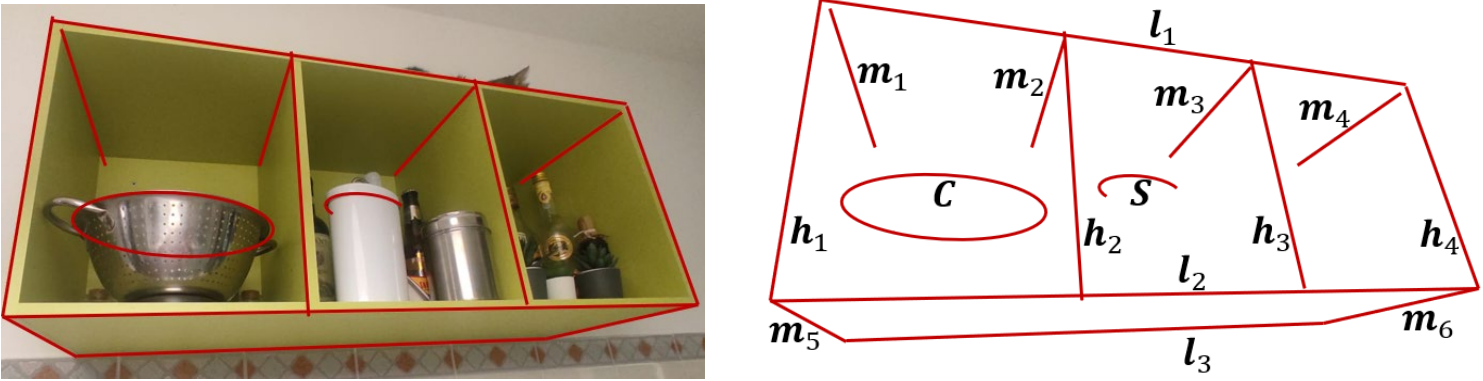
\includegraphics[width=\textwidth]{images/lines.png}
    \caption{Lines and curves needed to be extracted}
    \label{fig:lines}
\end{figure}

\noindent For both lines and curves, points were extracted (two for each line and five for each curve) and parameters were computed based on these points.

To extract the required points, a preprocessing step was applied to the image, followed by the Harris feature detection algorithm implemented in MATLAB. 
The Harris method was chosen for its ability to localize corners with sub pixel accuracy, with an empirically determined correspondence error typically less than one pixel. 
The preprocessing involved the following steps:
\begin{enumerate}
    \item Convert the image to a single channel (gray scale image).
    \item Apply a Gaussian filter to smooth edges.
    \item Detect edges using the Canny edge detection algorithm.
\end{enumerate}

After preprocessing, the Harris algorithm was applied to the Region of Interest (ROI) containing the desired points. 
Points were manually refined to ensure they accurately corresponded to vertices or lines of interest.

\subsection{Lines computation}
Lines were computed by imposing passage through pairs of points. In two dimensions, the cross product of two points, $\mathbf{p}_1$ and $\mathbf{p}_2$, yields the line equation:
\begin{equation}\mathbf{l}=\mathbf{p}_1 \times \mathbf{p}_2\end{equation}

\subsection*{MATLAB}
The script for feature extraction are in the following path: \\ 
\texttt{src/image\_analysis/1\_feature\_extraction/1\_lines\_extraction/main.m} \\
In this script, the points within the ROI containing perpendicular objects were extracted. 
Points close to the desired positions were manually refined. 
Key variables include:
\begin{itemize}
    \item \texttt{points}: contains all points used for line computation.
    \item \texttt{lines}: stores line parameters computed via cross product of point pairs.
    \item \texttt{curves\_points}: contains points used for curve computation in the subsequent script.
\end{itemize}
The extracted points and lines are shown in Figure~\ref{fig:ext_lines}.
\begin{figure}[!htb]%recommended float settings
    \centering
    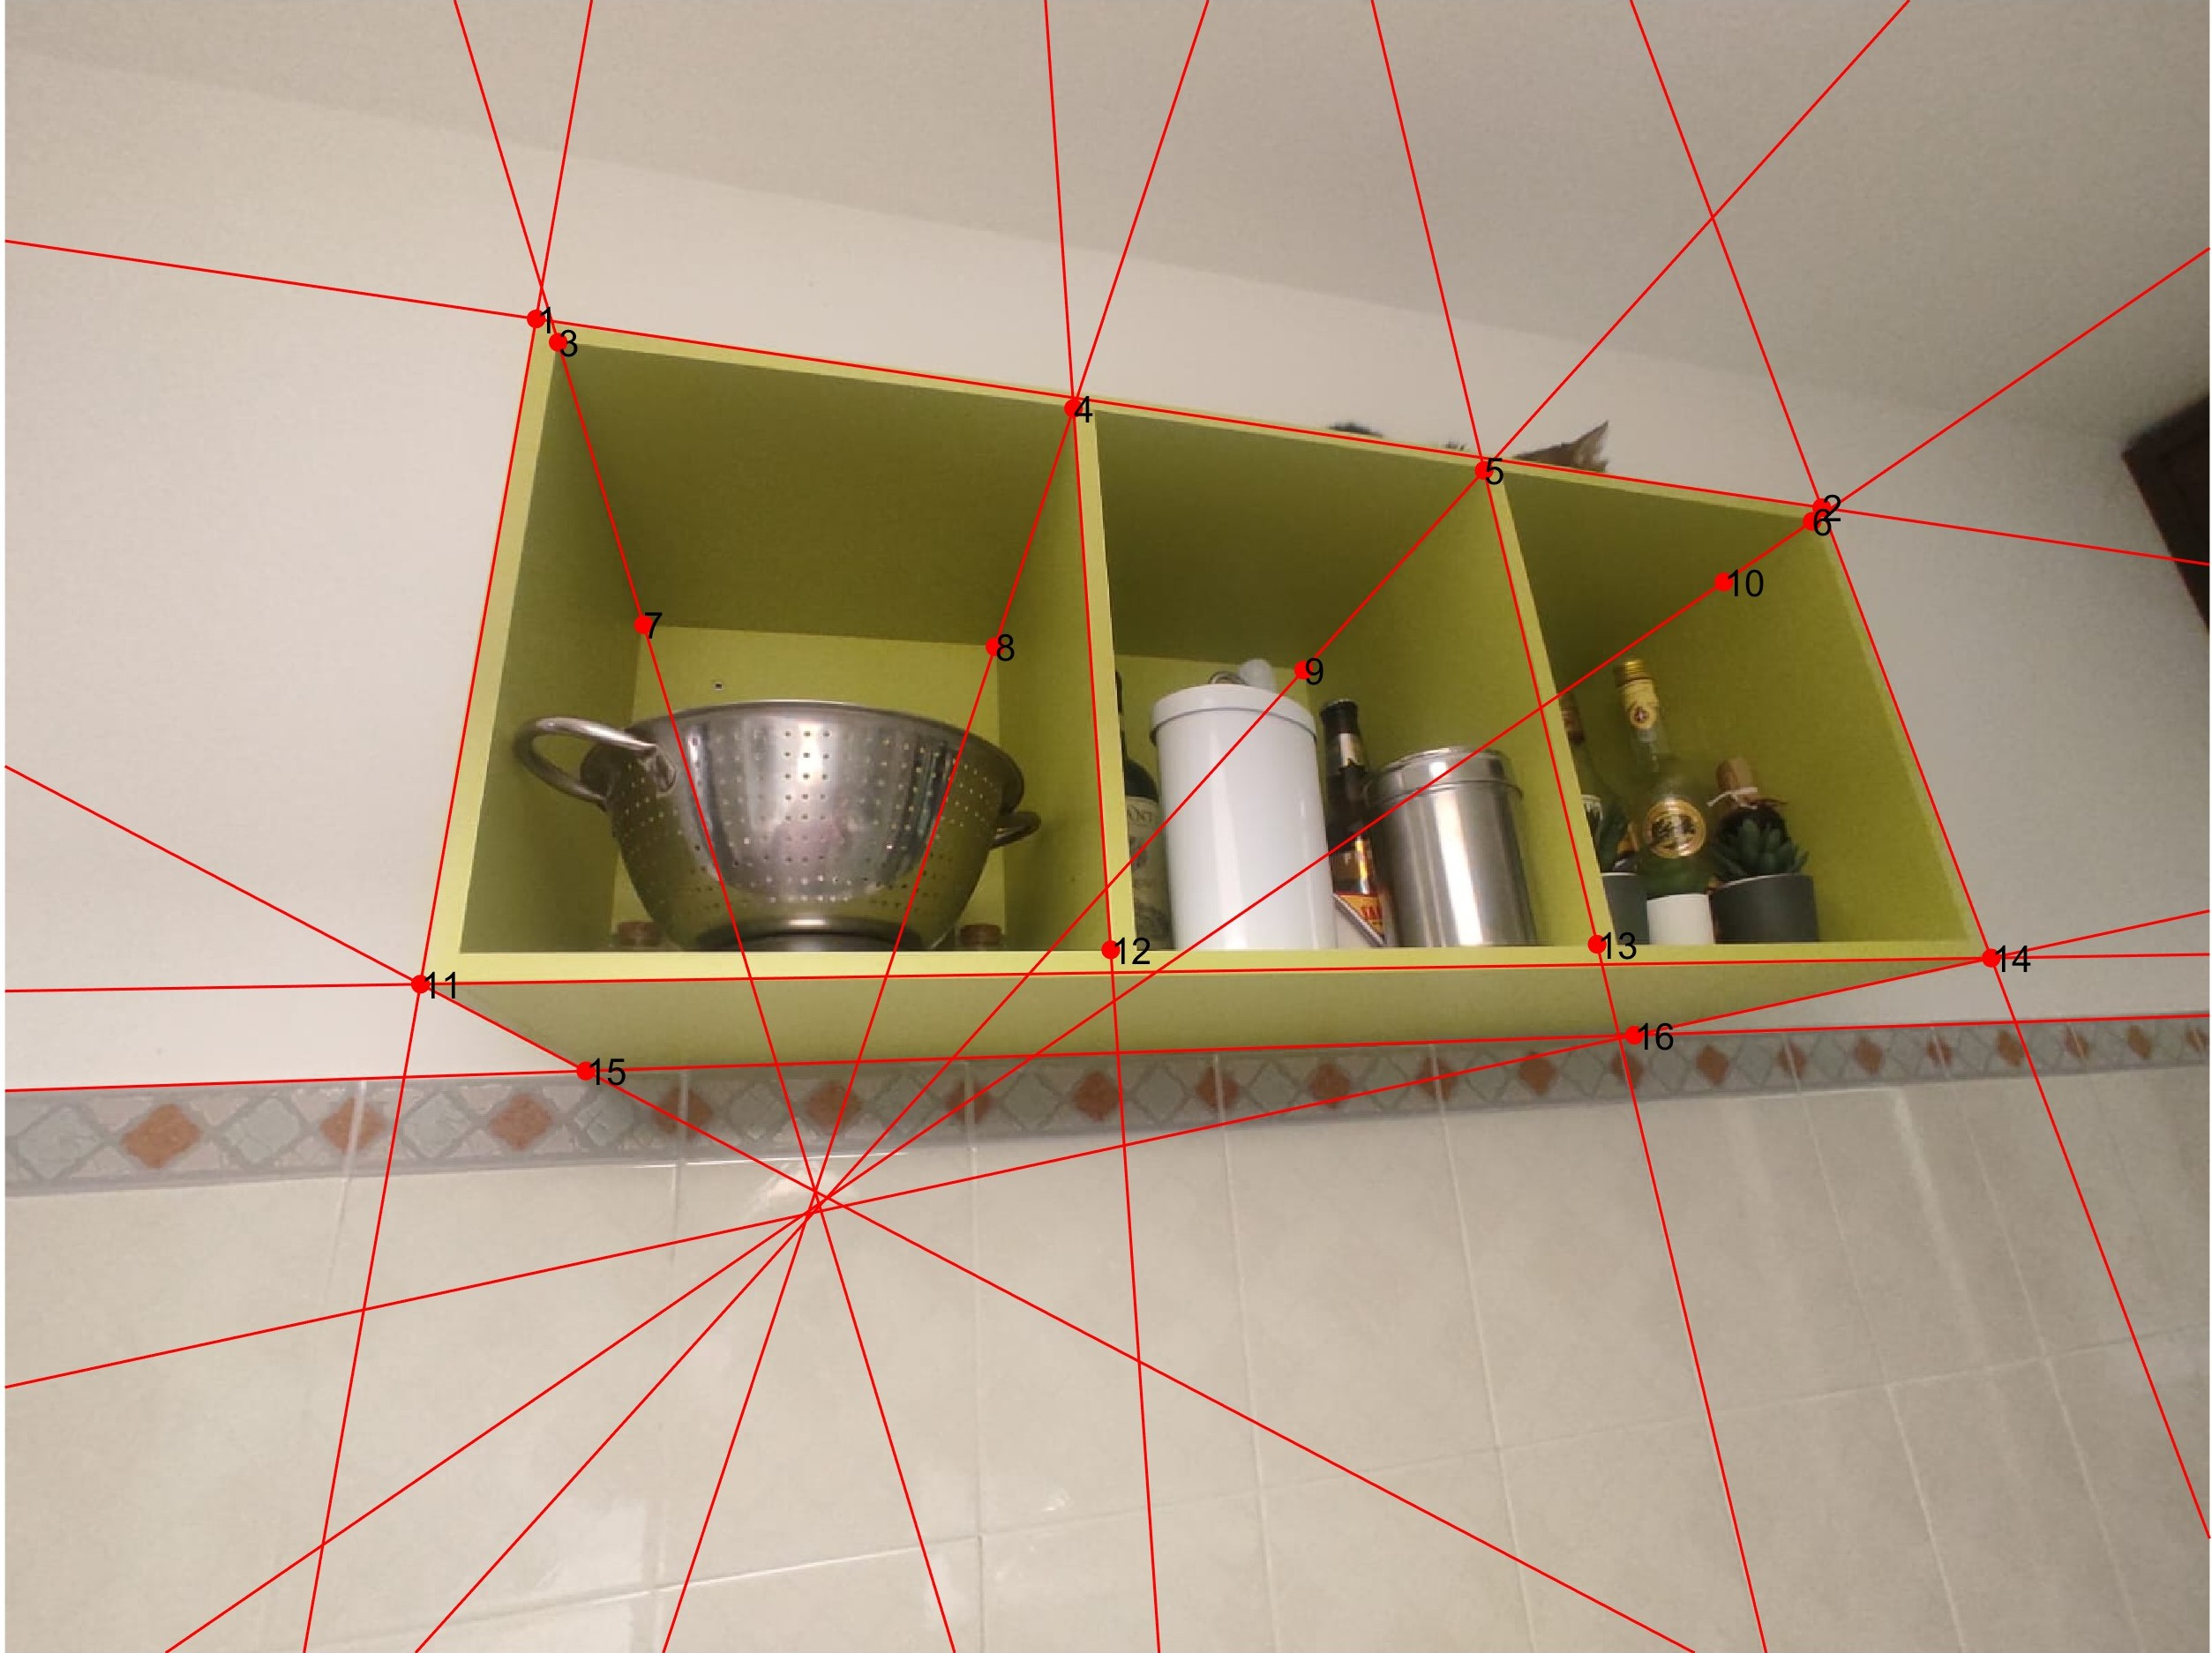
\includegraphics[width=0.5\textwidth]{images/ext_lines.jpg}
    \caption{Extracted points and lines}
    \label{fig:ext_lines}
\end{figure}

\subsection{Curves computation}
For curves, the general conic equation was used:
\begin{equation}ax^2 + by^2 + cxy + dx + ey + f = 0\end{equation}
Five points were used to form a system of equations. 
By computing the right null space of the matrix representing these equations and constraining the parameter $f$ to one, the conic coefficients were determined. 
The conic matrix was then constructed as follows:
\begin{equation}\mathbf{C} = \begin{bmatrix} a & \frac{b}{2} & \frac{d}{2} \\ \frac{b}{2} & c & \frac{e}{2} \\ \frac{d}{2} & \frac{e}{2} & f\end{bmatrix}\end{equation}

\subsection*{MATLAB}
The script for feature extraction are in the following path: \\ 
\texttt{src/image\_analysis/1\_feature\_extraction/2\_curves\_extraction/main.m} \\
This script imports the points identified in \texttt{lines\_detection} and applies similar steps for curve computation.
Singular Value Decomposition (SVD) was used to compute the right null space of matrix $\mathbf{A}$, representing the system of equations, to ensure robust and accurate results.
The extracted curves are shown in Figure~\ref{fig:ext_curves}.
\begin{figure}[!htb]%recommended float settings
    \centering
    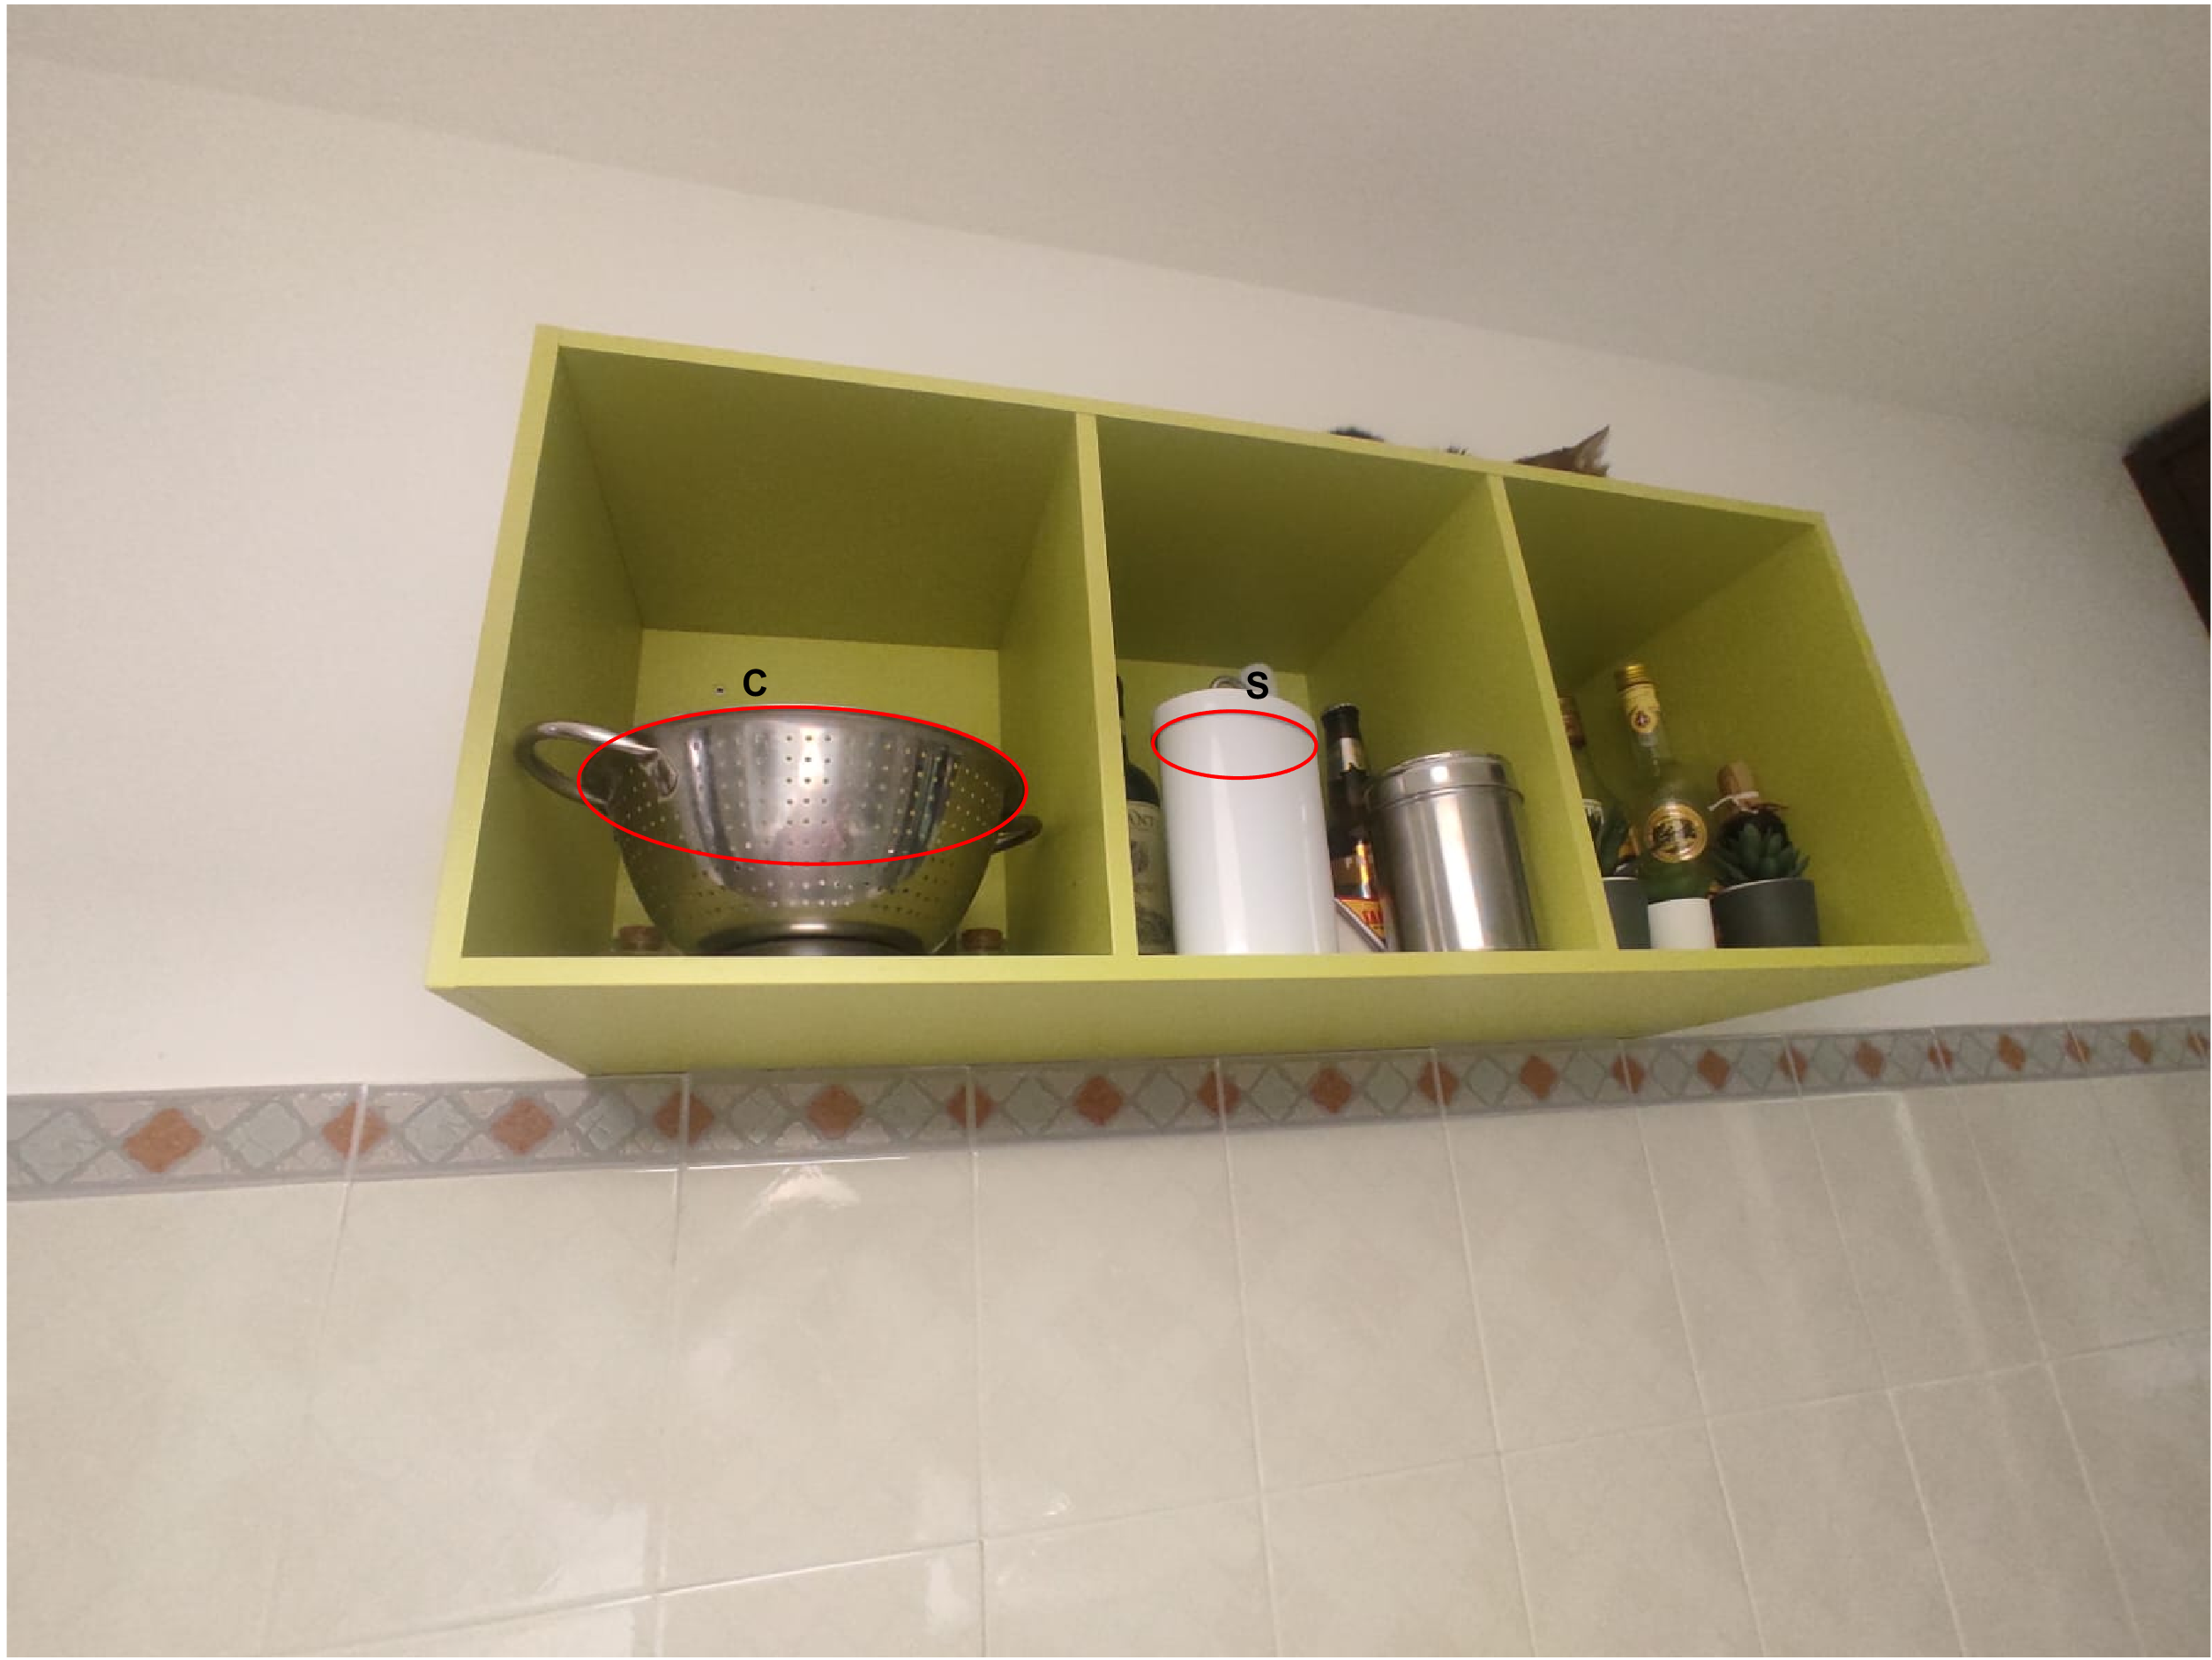
\includegraphics[width=0.5\textwidth]{images/ext_curves.png}
    \caption{Extracted curves}
    \label{fig:ext_curves}
\end{figure}

\section{Image Analysis}
This section outlines the steps required to analyze the image, including the processes for both camera calibration and localization. 
The operations performed here are critical for extracting accurate features, computing calibration parameters, and achieving precise localization of the camera in its environment.
\subsection{Horizontal vanishing line identification}
The goal of this task is to determine the vanishing line, denoted as $\mathbf{l}^\prime_{\infty}$, of the horizontal plane. 
This plane is defined by the length and depth of the object shown in Figure~\ref{fig:scene}.

\begin{figure}[!htb]%recommended float settings
    \centering
    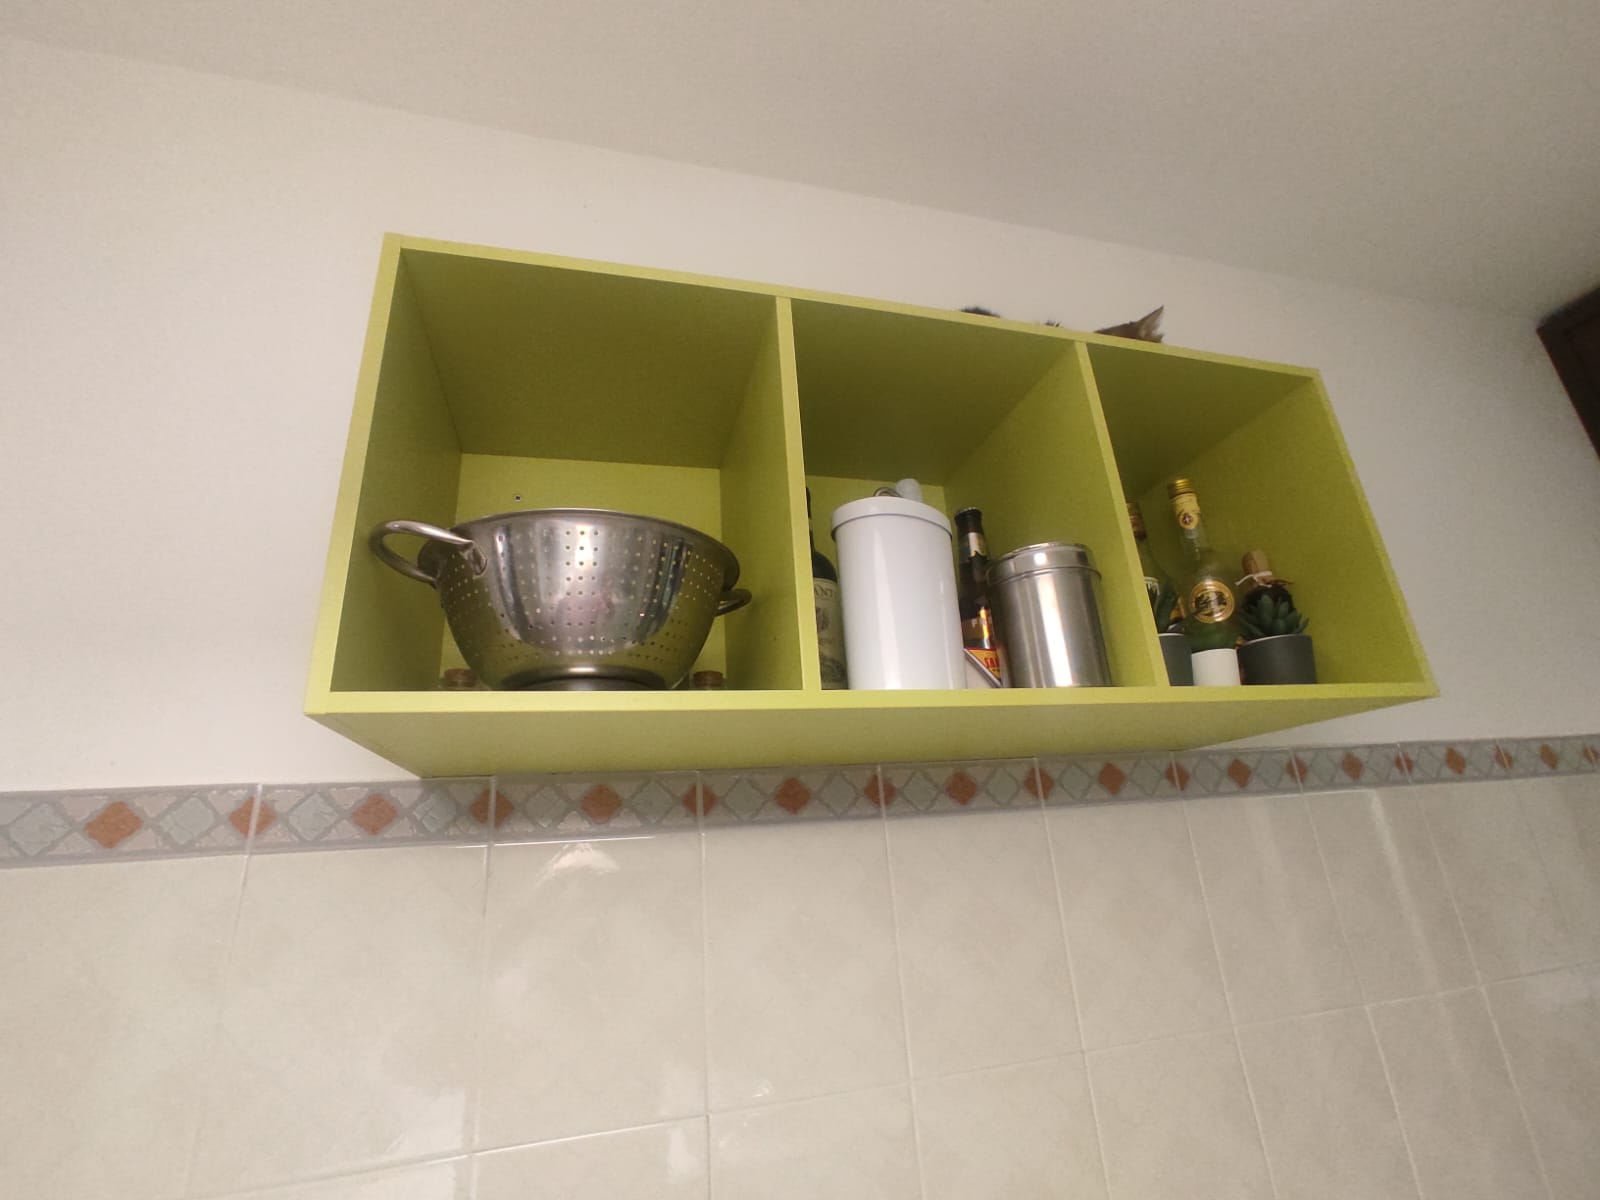
\includegraphics[width=0.5\textwidth]{images/scene.jpg}
    \caption{Image of the scene}
    \label{fig:scene}
\end{figure}

\noindent The horizontal plane is characterized by two sets of parallel lines: $\mathbf{l}_1$ and $\mathbf{l}_3$ for the length, and $\mathbf{m}_5$ and $\mathbf{m}_6$ for the depth.

To determine the vanishing points, we compute the intersections of these parallel lines in the image space. 
Parallel lines in the real world appear to converge at vanishing points in the image, as stated by the following theorem: the image of a set of parallel lines $\mathbf{n}_i$ is a set of concurrent lines $\mathbf{n}^\prime_i$ that intersect at a common point $\mathbf{p}^\prime$, referred to as the vanishing point of the direction of lines $\mathbf{n}_i$.

For the length and depth directions, the vanishing points are calculated as:
\begin{equation}\mathbf{p}_l=\mathbf{l}_1 \times \mathbf{l}_3\end{equation}
\begin{equation}\mathbf{p}_m=\mathbf{m}_5 \times \mathbf{m}_6\end{equation}

\noindent The coordinates of the vanishing points are expressed as:
\begin{equation}\mathbf{p}_l=\begin{bmatrix} x_l \\ y_l \\ w \end{bmatrix} \qquad \mathbf{p}_m=\begin{bmatrix} x_m \\ y_m \\ w \end{bmatrix}\end{equation}

The vanishing line for the horizontal plane, $\mathbf{l}^\prime_{\infty}$, is defined as the line connecting these two vanishing points. 
This line is computed as the cross product of $\mathbf{p}_l$ and $\mathbf{p}_m$:
\begin{equation}\mathbf{l}^\prime_{\infty}= \mathbf{p}_m^T \times \mathbf{p}_l^T=\begin{bmatrix} a \\ b \\ c \end{bmatrix}\end{equation}

\paragraph*{MATLAB}
The script for identifying vanishing points and the vanishing line is located at: \\ 
\texttt{src/image\_analysis/2\_theory\_implementation/1\_vanishing\_line/main.m} \\
In this script, previously extracted lines were imported, and vanishing points for all directions were computed, as they may be useful for later analysis.
The identified vanishing points are illustrated in Figure~\ref{fig:vanishing}, where $\mathbf{p}_l$, $\mathbf{p}_m$, and $\mathbf{p}_h$ (the vanishing point for the vertical facade) are labeled as 1, 2, and 3, respectively.

\noindent The calculated coordinates are as follows:
\begin{equation}\mathbf{p}_l=\begin{bmatrix}
    3,392.6958 \\ 673.49768 \\ 1
\end{bmatrix} \qquad \mathbf{p}_m=\begin{bmatrix}
    607.2928 \\ 876.4772 \\ 1
\end{bmatrix} \qquad \mathbf{p}_h=\begin{bmatrix}
    664.6947 \\ -1,370.4946 \\ 1
\end{bmatrix}\end{equation}

To compute the horizontal line at infinity, the line passing through $\mathbf{p}_l$ and $\mathbf{p}_m$ was determined using the cross product. 
The resulting line, shown in Figure~\ref{fig:vanishing}, has the following parameters:
\begin{equation}\mathbf{l}_{\infty}^\prime=\begin{bmatrix}
    a \\ b \\ c
\end{bmatrix}=\begin{bmatrix}
    -0.00007 \\ -0.0011 \\ 1
\end{bmatrix}\end{equation}
\begin{figure}[!htb]
    \centering
    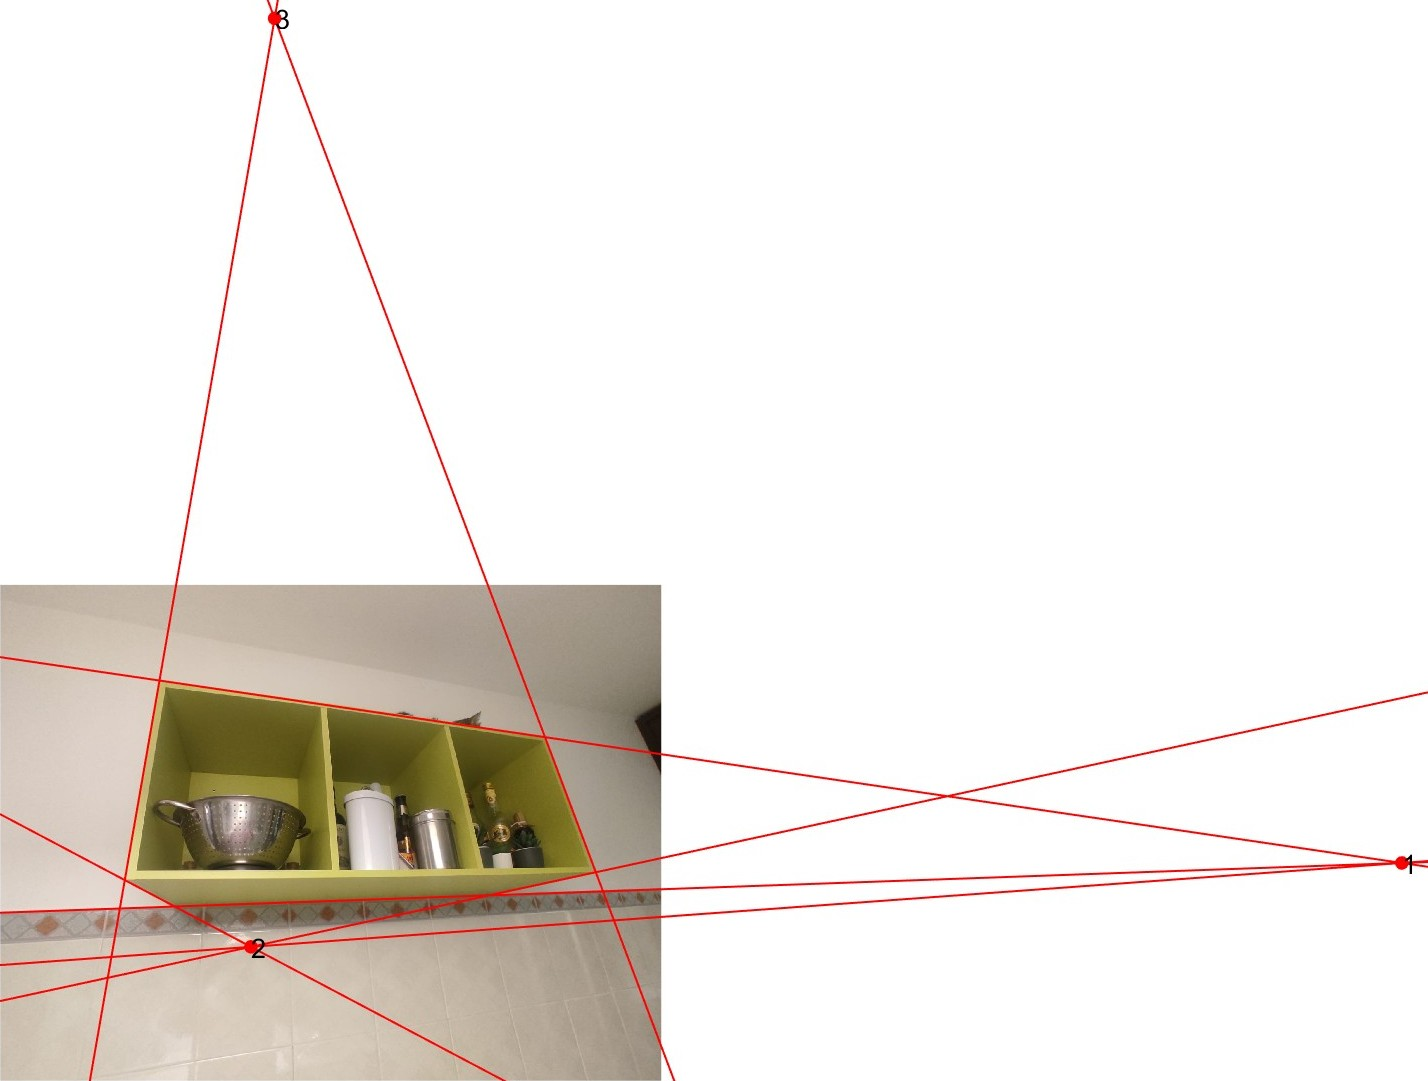
\includegraphics[width=0.5\linewidth]{images/vanishing.jpg}
    \caption{Vanishing points for depth, height, and length and vanishing line}
    \label{fig:vanishing}
\end{figure}

\subsection{Image rectification}
The objective of this section is to establish a rectification mapping for the horizontal plane analyzed earlier and subsequently compute the object's depth. 
This process is implemented using a stratified approach, starting with affine rectification followed by metric rectification.

From geometric theory, the line at infinity identified in the previous step must be mapped to the real line at infinity in the scene. 
Specifically, the line $\mathbf{l}^\prime_{\infty}$ in the image must be transformed back to $\mathbf{l}_{\infty}$:
\begin{equation}\mathbf{l}^\prime_{\infty}=\begin{bmatrix}
    a \\ b \\ c
\end{bmatrix}\xrightarrow[]{\text{mapped back to}}\begin{bmatrix}
    0 \\ 0 \\ 1
\end{bmatrix}=\mathbf{l}_{\infty}\end{equation}
To achieve this, we construct a homography matrix that aligns $\mathbf{l}^\prime_{\infty}$ with $\mathbf{l}_{\infty}$:
\begin{equation}\mathbf{H}_{\text{aff}}=\begin{bmatrix}
    1 & 0 & 0 \\
    0 & 1 & 0 \\
    a & b & c
\end{bmatrix}\end{equation}
By applying this transformation matrix to all pixels in the image, we obtain a rectified version of the scene.

Using the stratified approach, we proceed to the metric rectification step. 

Since identifying two pairs of orthogonal lines was not feasible, we utilized the circumference $\mathbf{C}$ to reconstruct the metric homography.
We began by applying the affine homography to the circumference matrix, yielding the matrix $\mathbf{Q}$ in the affine space:
\begin{equation}\mathbf{Q} = \begin{bmatrix} a_q & \frac{b_q}{2} & \frac{d_q}{2} \\ \frac{b_q}{2} & c_q & \frac{e_q}{2} \\ \frac{d_q}{2} & \frac{e_q}{2} & f_q\end{bmatrix}\end{equation}
From $\mathbf{Q}$, we extracted the primary axes and the rotation angle $\alpha$ of the curve. 
These parameters allowed us to reconstruct the homography matrix $\mathbf{H}_{\text{met}}$, enabling metric rectification.
The process involved rescaling the axes of the curve to make them unitary.

First, we computed the scaling matrix $\mathbf{S}$, which adjusts the axes:
\begin{equation}
    \mathbf{S} = \begin{bmatrix}
        1 & 0 \\ 0 & \frac{a_q}{b_q}
    \end{bmatrix}
\end{equation}
Next, we applied the rotation matrix $\mathbf{R}$ to account for the ellipse's orientation:
\begin{equation}
    \mathbf{R}=\begin{bmatrix}
        \cos(\alpha) & -\sin(\alpha) \\ \sin(\alpha) & \cos(\alpha)
    \end{bmatrix}
\end{equation} 
Combining these, the reduced metric rectification matrix is obtained as:
\begin{equation}
    \mathbf{H}_{\text{red}}= \mathbf{RSR}^{-1}
\end{equation}
Finally, we extended $\mathbf{H}_{\text{red}}$ to include the projective space, producing the full metric rectification matrix:
\begin{equation}
    \mathbf{H}_{\text{met}}=\begin{bmatrix}
        \mathbf{H}_{\text{red}} & \mathbf{0} \\
        \mathbf{0} & 1
    \end{bmatrix}
\end{equation}
This matrix $\mathbf{H}_{\text{met}}$ can now be used to achieve metric rectification of the image.

Now, we reconstructed the final homography between the initial image and the metric rectified by multiplying the two homographies: 
\begin{equation}
    \mathbf{H} = \mathbf{H}_{\text{met}} \mathbf{H}_{\text{aff}}
\end{equation}

The final step is to compute the object's depth using the metric rectified image. 
Assuming the object's length is known and unitary, we measure both the length and depth directly on the rectified image using Euclidean distances between corresponding points. 

\noindent The real-world depth is calculated as:
\begin{equation}\text{real depth}=\dfrac{\text{depth}}{\text{width}} \cdot 1\end{equation}

\paragraph*{MATLAB}
The MATLAB script for finding the vanishing points and lines is located in the following path: \\ 
\texttt{src/image\_analysis/2\_theory\_implementation/2\_rectification/main.m} \\

For the initial rectification, the line at infinity for the horizontal plane found earlier was used. 
The rectification matrix obtained is:
\begin{equation}\mathbf{H}_{\text{aff}} = \begin{bmatrix}
    1 & 0 & -0.0007 \\ 
    0 & 1 & -0.0011 \\ 
    0 & 0 &  1\\ 
\end{bmatrix}\end{equation}
\noindent The rectified image obtained using this homography matrix is shown in Figure \ref{fig:rectified}.
\begin{figure}[!htb]%recommended float settings
    \centering
    \includegraphics[width=0.5\linewidth]{images/rectified.jpg}
    \caption{Affine rectification of the image}
    \label{fig:rectified}
\end{figure}

After applying the affine homography $\mathbf{H}_{\text{aff}}$ to the conic $\mathbf{C}$, we extracted all the parameters from the resulting matrix $\mathbf{Q}$. 
From $\mathbf{Q}$, we determined the axes and rotation angle of the ellipse, which allowed us to construct the metric homography matrix $\mathbf{H}_{\text{met}}$ by combining the rotation matrix $\mathbf{R}$ and the scaling matrix $\mathbf{S}$.
The resulting matrix is:
\begin{equation}\mathbf{H}_{\text{met}}=\begin{bmatrix}
    1.3899 & -0.5937 & 0 \\
    -0.5937 & 1.9042 & 0 \\
    0 & 0 & 1
\end{bmatrix}\end{equation}
Using this, we reconstructed the final homography $\mathbf{H}$ between the initial image and the metric-rectified image, which is given by:
\begin{equation}\mathbf{H}=\begin{bmatrix}
    1.3899 & -0.5937 & 0 \\
   -0.5937 & 1.9042 & 0 \\
   -0.0001 & -0.0011 & 1
\end{bmatrix}\end{equation}
\noindent The rectified image obtained using this homography is shown in Figure \ref{fig:metric}.
\begin{figure}[!htb]%recommended float settings
    \centering
    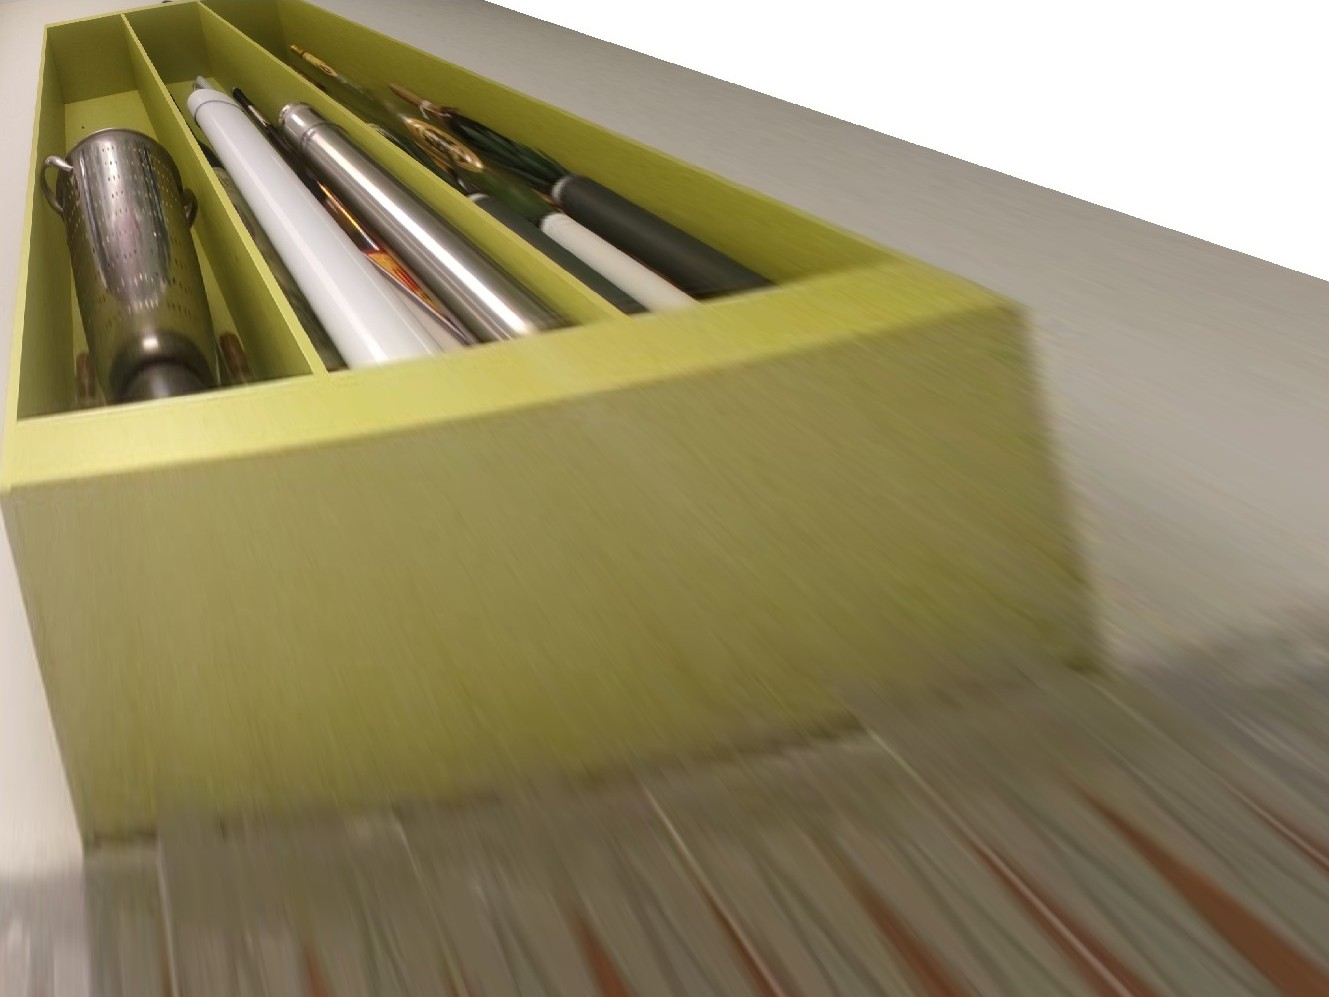
\includegraphics[width=0.5\linewidth]{images/metric.jpg}
    \caption{Metric-rectified image}
    \label{fig:metric}
\end{figure}

After measuring the length and depth, the depth-to-length ratio was found to be:
\begin{equation}\text{real depth}=\dfrac{\text{depth}}{\text{width}} \cdot 1 = \dfrac{\text{4,320.6862}}{\text{12,127.8589}} = 0.3562\end{equation}
The checked lines confirmed orthogonality, achieving the desired rectification and depth calculation results.

\subsection{Calibration}
The aim of this section is to compute the calibration matrix $\mathbf{K}$, which encapsulates the intrinsic parameters of the camera. 
These parameters are essential for mapping 3D scene points into the 2D image plane. 
The calibration matrix $\mathbf{K}$ is defined as:
\begin{equation}\mathbf{K} = \begin{bmatrix} f_x & s & u_0 \\ 0 & f_y & v_0 \\ 0 & 0 & 1 \end{bmatrix}\end{equation}
Here: 
\begin{itemize}
    \item $f_x$ and $f_y$ are the effective focal lengths along the $x$ and $y$ axes, respectively.
    \item $u_0$ and $v_0$ represent the coordinates of the principal point, which is the optical center in the image.
    \item $s$ is the skew parameter, representing the angle between the $x$ and $y$ axes of the image. 
        For most modern cameras, the axes are orthogonal, and the skew parameter is assumed to be $s = 0$.
\end{itemize}

The computation of $\mathbf{K}$ relies on the Image of the Absolute Conic (IAC), represented by the symmetric matrix $\boldsymbol{\omega}$:
\begin{equation} \label{eqn:iac} \boldsymbol{\omega} = \begin{bmatrix} a & 0 & b \\ 0 & 1 & c \\ b & c & d \end{bmatrix}\end{equation}
The IAC encodes the intrinsic parameters of the camera and is pivotal for recovering $\mathbf{K}$.

To estimate $\boldsymbol{\omega}$, geometric constraints are imposed based on the vanishing points, line at infinity, and the combined homography matrix.
hese elements include:
\begin{enumerate}
    \item \textit{Vanishing points}: $\mathbf{p}_h$, $\mathbf{p}_m$, and $\mathbf{p}_l$.
    \item \textit{Metric homography matrix}: complete homography matrix from original image to the metric reconstructed one. 
    \item \textit{Line at the infinity}: the line at infinity of the horizontal plane.
\end{enumerate}
\noindent The constraints imposed on $\boldsymbol{\omega}$ are formulated as follows:
\begin{equation}
\label{eqn:constraints}
\begin{cases}
    \left[\mathbf{l}_{\infty}^{\prime T}\right] \times \boldsymbol{\omega} \times \mathbf{p}_h = 0 \\
    \mathbf{p}_m^T \times \boldsymbol{\omega} \times \mathbf{p}_l = 0  \\
    \mathbf{h}_1^T \times \boldsymbol{\omega} \times \mathbf{h}_1 - \mathbf{h}_2^T \times \boldsymbol{\omega} \times \mathbf{h}_2 = 0 \\
    \mathbf{h}_1^T * \boldsymbol{\omega} * \mathbf{h}_2 = 0
\end{cases}\end{equation}
Here, $\mathbf{h}_1$ and $\mathbf{h}_2$ are the first and second columns of the homography matrix $\mathbf{H}$. 

\noindent These constraints form a system of linear equations that is solved to determine the elements $a$, $b$, $c$, and $d$ of the IAC matrix $\boldsymbol{\omega}$.
\noindent Once the IAC matrix $\boldsymbol{\omega}$ is determined, the intrinsic camera parameters are computed using the following formulas:
\begin{equation}
\begin{cases}
    f_x = \sqrt{d - \alpha^2 \cdot u_0^2 - v_0^2} \\
    f_y = \frac{f_y}{\alpha} \\
    u_0 = - \frac{b}{\alpha^2} \\
    v_0 = - c
\end{cases}
\end{equation}
Here, $\alpha = \sqrt{a}$. 
With these parameters, we can construct the final calibration matrix $\mathbf{K}$.

\paragraph*{MATLAB}
The calibration matrix computation script is located at: \\ 
\texttt{src/image\_analysis/2\_theory\_implementation/3\_calibration/main.m} \\
The workflow in the script is as follows:
\begin{enumerate}
    \item Import the vanishing points, the line at infinity for the horizontal plane, and the transformation matrix $\mathbf{H}$.
    \item Normalize the inputs to mitigate numerical inaccuracies.
    \item Formulate the system of equations based on the constraints in Equation \eqref{eqn:constraints}.
    \item Solve the system.
\end{enumerate}
The solution of the system returned the following IAC matrix $\boldsymbol{\omega}$:
\begin{equation} \boldsymbol{\omega} = \begin{bmatrix} 
    0.9286 & 0 & -761.7285 \\
    0 & 1 & -612.4760 \\
    -761.7285 & -612.4760 & 1,492,707.0013
\end{bmatrix}
\end{equation}
\noindent Using this IAC, the intrinsic camera parameters were computed, resulting in the calibration matrix $\mathbf{K}$:
\begin{equation}\mathbf{K} = \begin{bmatrix} 
    728.4366 & 0 & 820.3127 \\
    0 & 701.94345 & 612.4760 \\ 
    0 & 0 & 1 
\end{bmatrix}\end{equation}

\subsection{Facade reconstruction}
The key idea here is to identify the image of the circular points by intersecting the line at infinity for the vertical plane, $\mathbf{l}_{v\infty}^\prime$, with the IAC $\boldsymbol{\omega}$. 
These circular points are crucial for rectifying the image and performing metric measurements.

To determine the image of the circular points, we impose the condition that the vanishing line of the vertical plane passes through the IAC. 
This leads to the following system of equations:
\begin{equation}
\label{eqn:iac2}
\begin{cases}
    \boldsymbol{\omega}_{11} x^2 + 2  \boldsymbol{\omega}_{12}  x  y + \boldsymbol{\omega}_{22}  y^2 + 2  \boldsymbol{\omega}_{13} x + 2  \boldsymbol{\omega}_{23}  y + \boldsymbol{\omega}_{33} = 0 \\ 
    \mathbf{l}_{\infty}^\prime(1)  x + \mathbf{l}_{\infty}^\prime(2)  y + \mathbf{l}_{\infty}^\prime(3) = 0;
\end{cases}\end{equation}
By solving this system, the two circular points, denoted as $\mathbf{I}$ and  $\mathbf{J}$, are obtained. 
These points lie on the conic defined by the IAC.

Using the circular points, the image of the dual conic $\mathbf{imDCCP}$ is computed as: 
\begin{equation}\mathbf{imDCCP}=\mathbf{IJ}^T+\mathbf{JI}^T\end{equation}
\noindent This dual conic is then used to compute the homography that maps the current image to a canonical position, where metric properties like distances can be measured.

\noindent To align the image to the canonical position, the following steps are performed:
\begin{enumerate}
    \item Perform Singular Value Decomposition (SVD) on $\mathbf{imDCCP}$.
    \item Compute the homography matrix $\mathbf{H}$ as:
        \begin{equation}\mathbf{H}=\left(\mathbf{U}\sqrt{\mathbf{D}}\right)^{-1}\end{equation}
\end{enumerate}
The homography $\mathbf{H}$ is applied to the image and the selected points used for measuring dimensions.

After applying the transformation, the height and length of the facade are computed as the Euclidean distance between respective pairs of points. 
The real height of the facade is determined using the ratio:
\begin{equation}\text{real height}=\dfrac{\text{height}}{\text{length}} \cdot 1 \end{equation}

\paragraph*{MATLAB}
The MATLAB implementation for this process is located at: \\ 
\texttt{src/image\_analysis/2\_theory\_implementation/4\_vertical\_reconstruction/main.m} \\
The script includes the computation of the the line at infinity $\mathbf{l}_{v\infty}^\prime$, and importing the previously computed IAC $\boldsymbol{\omega}$. 
Those variables are used to solve the system to recover the circular points:
\begin{equation}\mathbf{I}=\begin{bmatrix}
    1,758.8524-1,337.0425i \\ -550.6820-1,001.7975i \\ 1
\end{bmatrix} \qquad \mathbf{J}=\begin{bmatrix}
    1,758.8524+1,337.0425i \\ -550.6820+1,001.7975i \\ 1
\end{bmatrix}\end{equation}
From these, $\mathbf{imDCCP}$ is derived as:
\begin{equation}
\mathbf{imDCCP}= \begin{bmatrix}
    0.4632 & -0.8186 & 0.0006 \\ 
    -0.8186 & -0.2484 & -0.0002 \\ 
    0.0006 & -0.0002 & 0.000003
\end{bmatrix}
\end{equation}
Finally, the homography matrix is computed:
\begin{equation}\mathbf{H}=\begin{bmatrix}
     -0.8362 & 0.5484 & -0.0006 \\ 
     -0.6188 & -0.9437 & 0.0003 \\ 
     -0.0004 & 0.0005 & 1
\end{bmatrix}\end{equation}
Applying the homography yielded the rectified facade, as shown in Figure \ref{fig:ext_height}. 

\noindent For better visualization, the image was rotated, and points were manually extracted for dimension measurements (Figure \ref{fig:ext_height}).
\begin{figure}[!htb]
    \centering
    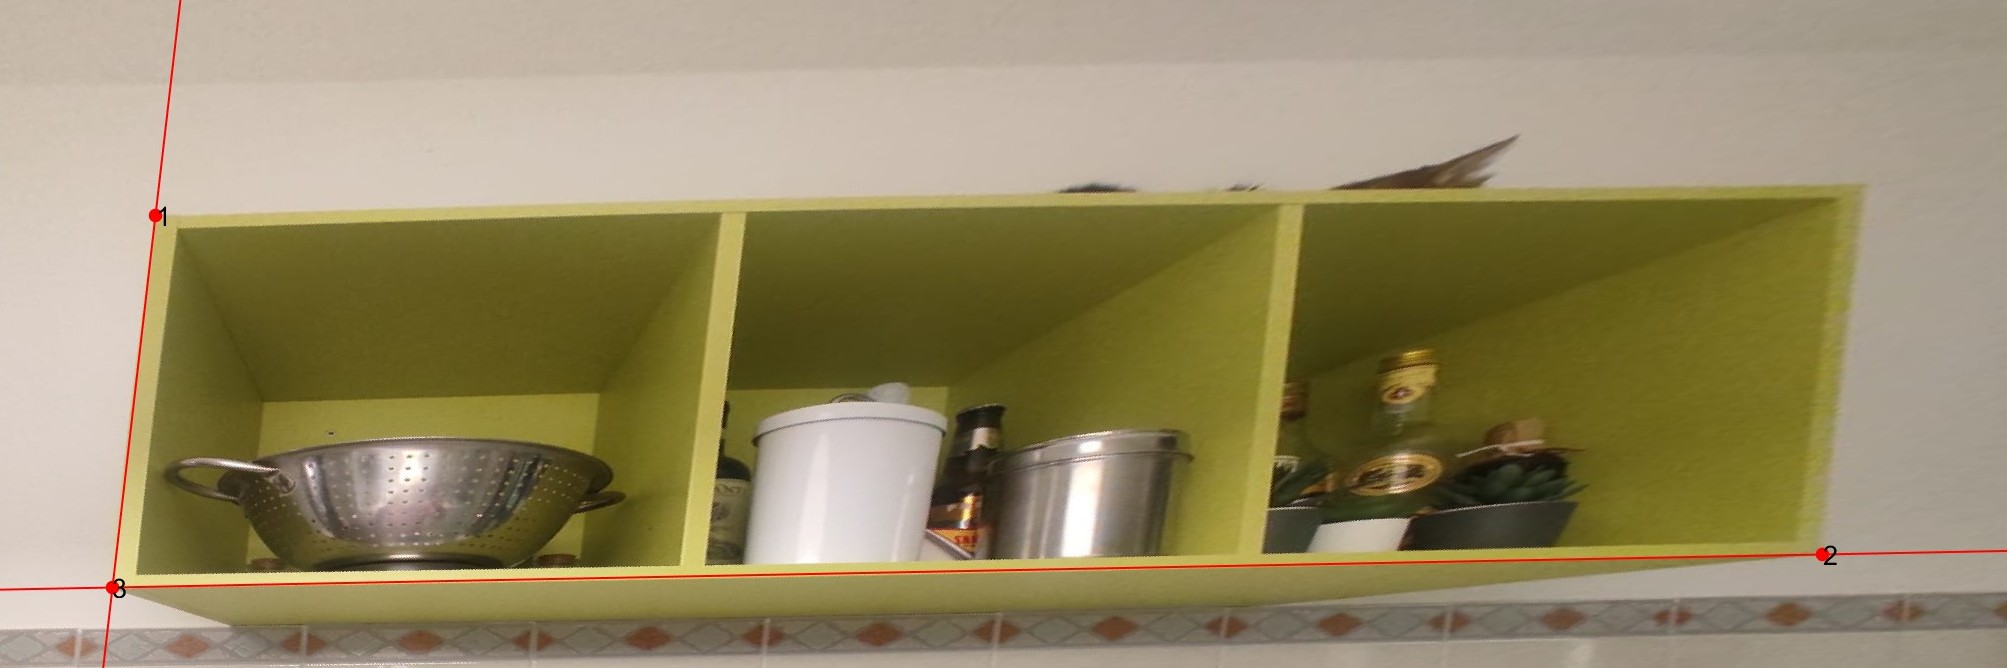
\includegraphics[width=0.5\linewidth]{images/ext_height.jpg}
    \caption{Extracted length and height}
    \label{fig:ext_height}
\end{figure}
The ratio between height and length is: 
\begin{equation}\text{real height}=\dfrac{\text{height}}{\text{length}} \cdot 1 =\dfrac{374.4769}{1,710.3184} = 0.2189 \end{equation}
The angle between the computed lines is $82.3008^\circ$, indicating a small deviation from orthogonality. 
This discrepancy arises because of the limited resolution of the image and the numerical imprecision due to the computations.

\subsection{Curve identification}
The goal of this step was to extract at least a dozen points from the unknown curve $\mathbf{S}$. 
Two potential methods were considered for this task:
\begin{enumerate}
    \item \textit{Harris detection algorithm}: a feature detection method that identifies corner-like features on the image.
    \item \textit{Random sampling from the conic equation}: this approach extracts points directly from the conic equation derived during the feature detection step.
\end{enumerate}
The second method was chosen, as it ensures that all selected points lie precisely on the same curve $\mathbf{S}$.
 Furthermore, this approach facilitates the approximation of points located on non-visible sections of the curve, offering a more complete representation of the geometry.

The conic equation provided a parametric framework for identifying candidate points on the curve. 
By sampling random points, the algorithm verified their validity by ensuring they satisfied the mathematical definition of the curve. 
This iterative process was repeated until the desired number of points (twelve) was successfully identified. 
The selected method not only guarantees consistency in point placement but also addresses the challenges posed by occluded or partially visible regions of the object.

We also transformed the points in the metric and vertical reconstructions by simply applying the transformation: 
\begin{equation}
    \mathbf{point}_{\text{transformed}} = \mathbf{point}_{\text{original}}\mathbf{H}
\end{equation}

\paragraph*{MATLAB}
The MATLAB implementation for curve point estimation is located in: \\ 
\texttt{src/image\_analysis/2\_theory\_implementation/5\_curve\_point\_estimation/main.m} \\
In this script, the number of points to be extracted is specified, and a fixed seed is set for the random number generator to ensure the reproducibility of results. 
The function \texttt{generate\_conic\_points} is used to sample points from the conic equation. 
Each sampled point is verified to ensure it satisfies the equation of the curve $\mathbf{S}$. 
Points that do not meet this criterion are discarded, and the process is repeated until the required number of points is obtained. 
Once the points are identified, they are visualized in the original image coordinate space to confirm their placement. 
The extracted points are illustrated in Figure \ref{fig:curve_points}.
\begin{figure}[!htb]%recommended float settings
    \centering
    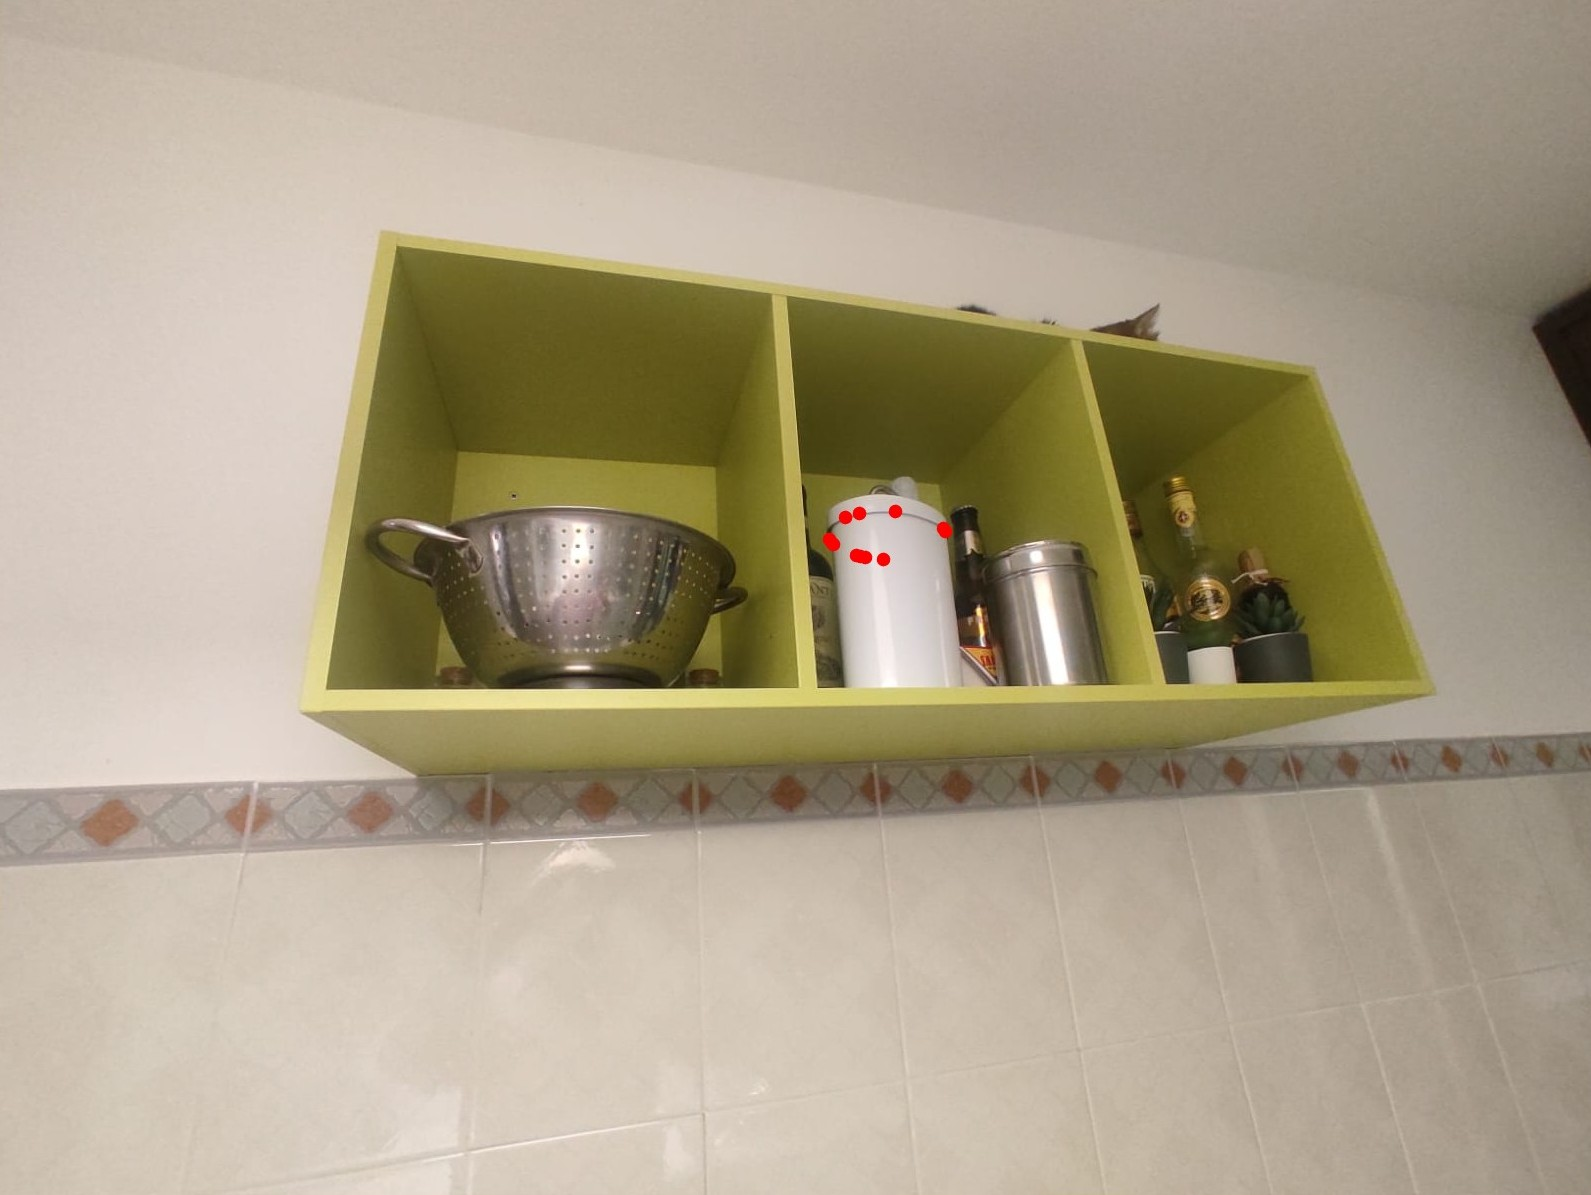
\includegraphics[width=0.5\linewidth]{images/curve_points.jpg}
    \caption{Extracted points for the curve $\mathbf{S}$}
    \label{fig:curve_points}
\end{figure}

\noindent While the points are extracted in the original image coordinate space, their locations can be seamlessly transformed into alternate coordinate systems using the corresponding homography matrix $\mathbf{H}$ with the equation described before. 
With the homographies found previously we obtained the results shown in Figure \ref{fig:poi}.
\begin{figure}[!htb]
    \centering
    \begin{minipage}{0.5\linewidth}
        \centering
        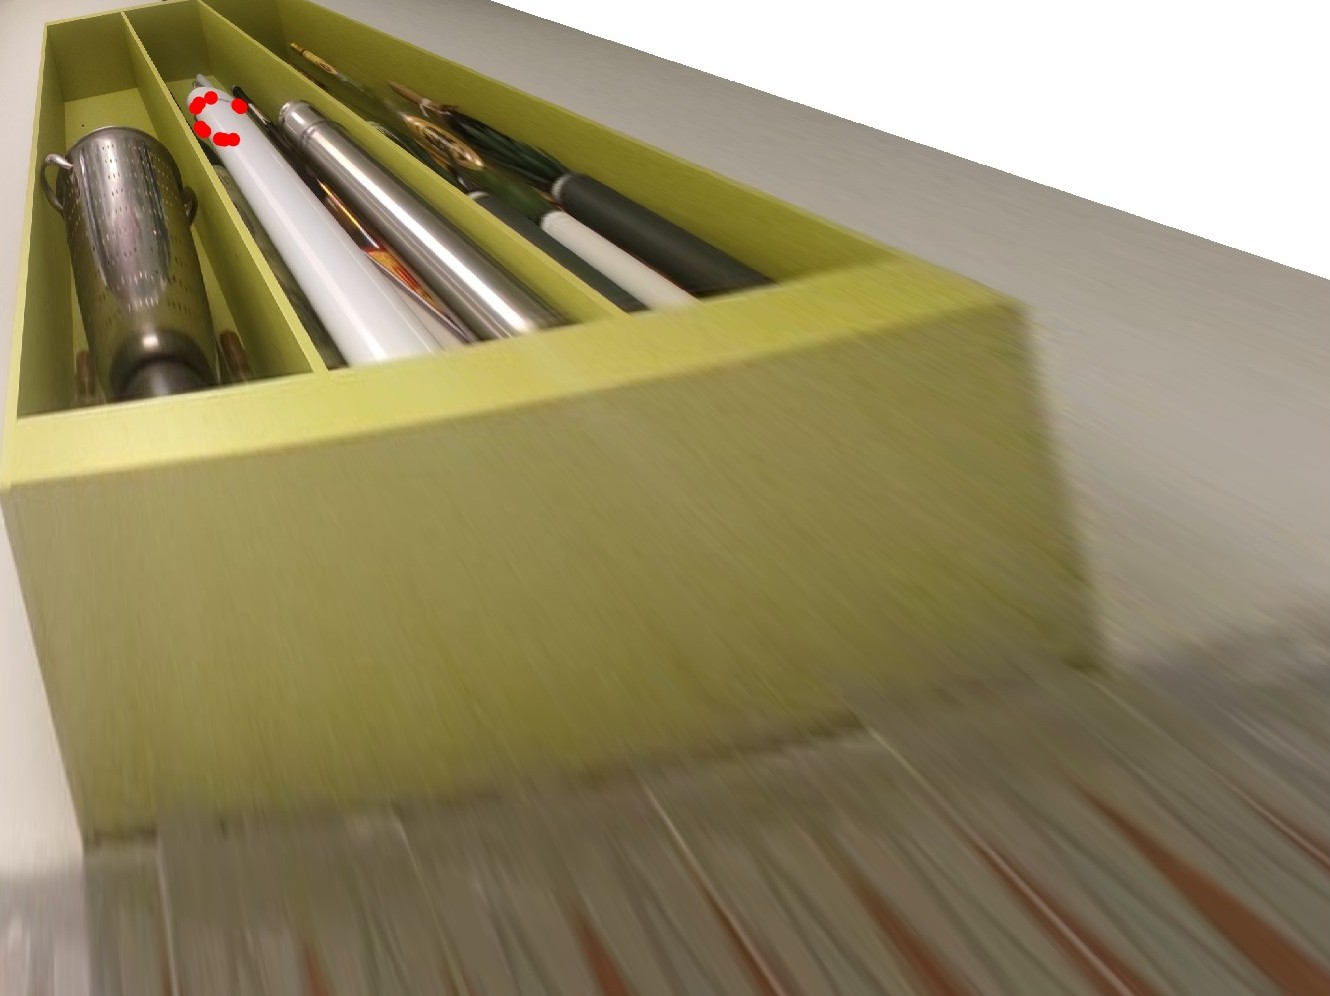
\includegraphics[width=\linewidth]{images/points_rec_1.jpg}
    \end{minipage}%
    \begin{minipage}{0.5\linewidth}
        \centering
        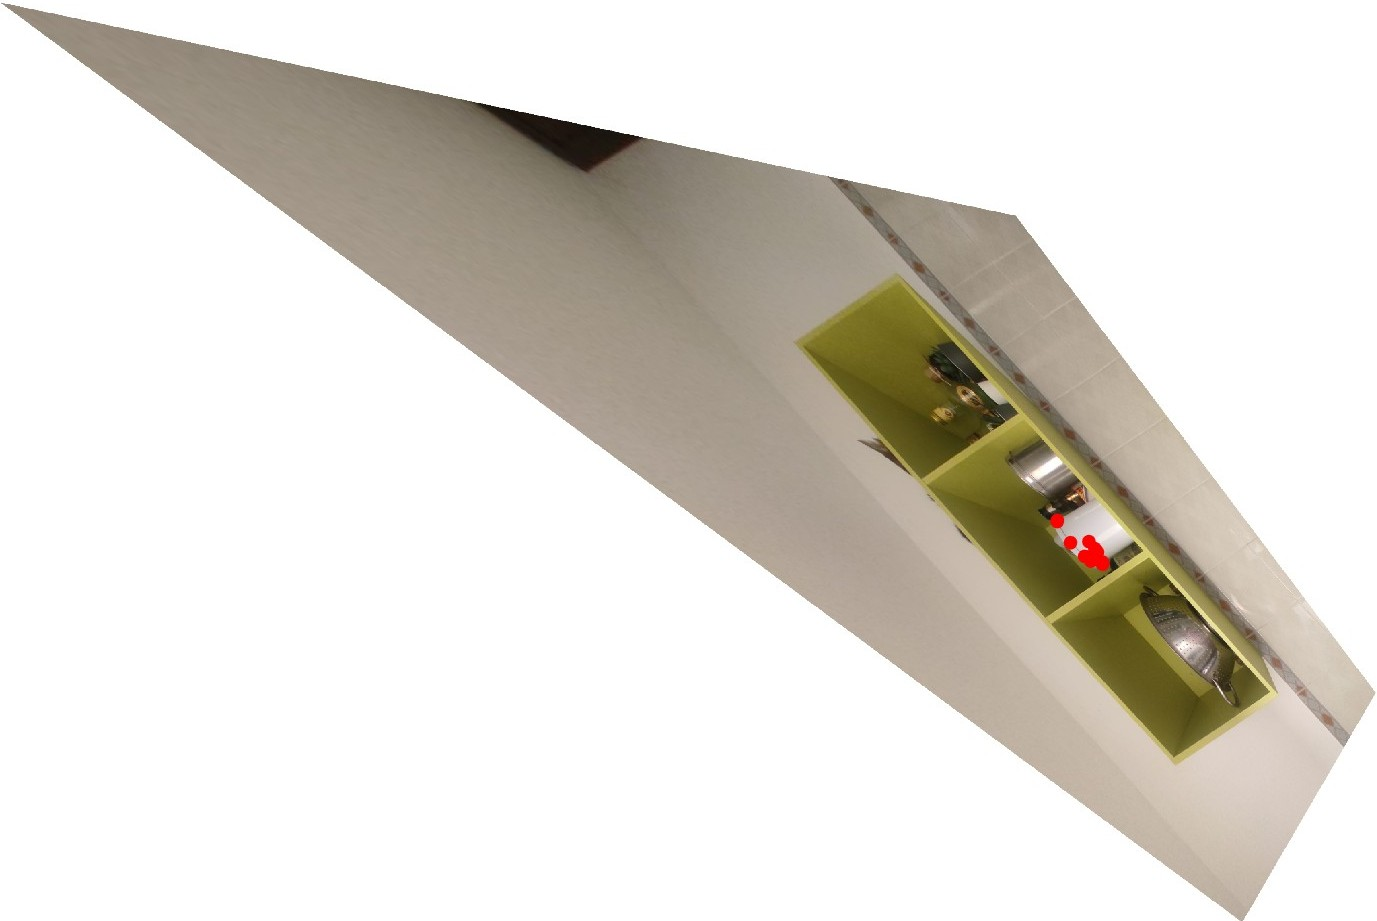
\includegraphics[width=\linewidth]{images/points_rec_2.jpg}
    \end{minipage}
    \caption{Metric rectification and vertical reconstructed images with points}
    \label{fig:poi}
\end{figure}

\subsection{Localization}
In this task, the goal was to determine the relative position of the camera with respect to a reference frame located at the bottom-left corner of the vertical facade shown in Figure~\ref{fig:world}.
\noindent  The camera's position was computed using the known dimensions of the vertical facade, including its length-height ratio, and the homographies required for metric reconstruction. 
With the calibration matrix $\mathbf{K}$, the image data, and the facade's geometric properties, the camera's position was obtained.
\begin{figure}[!htb]
    \centering
    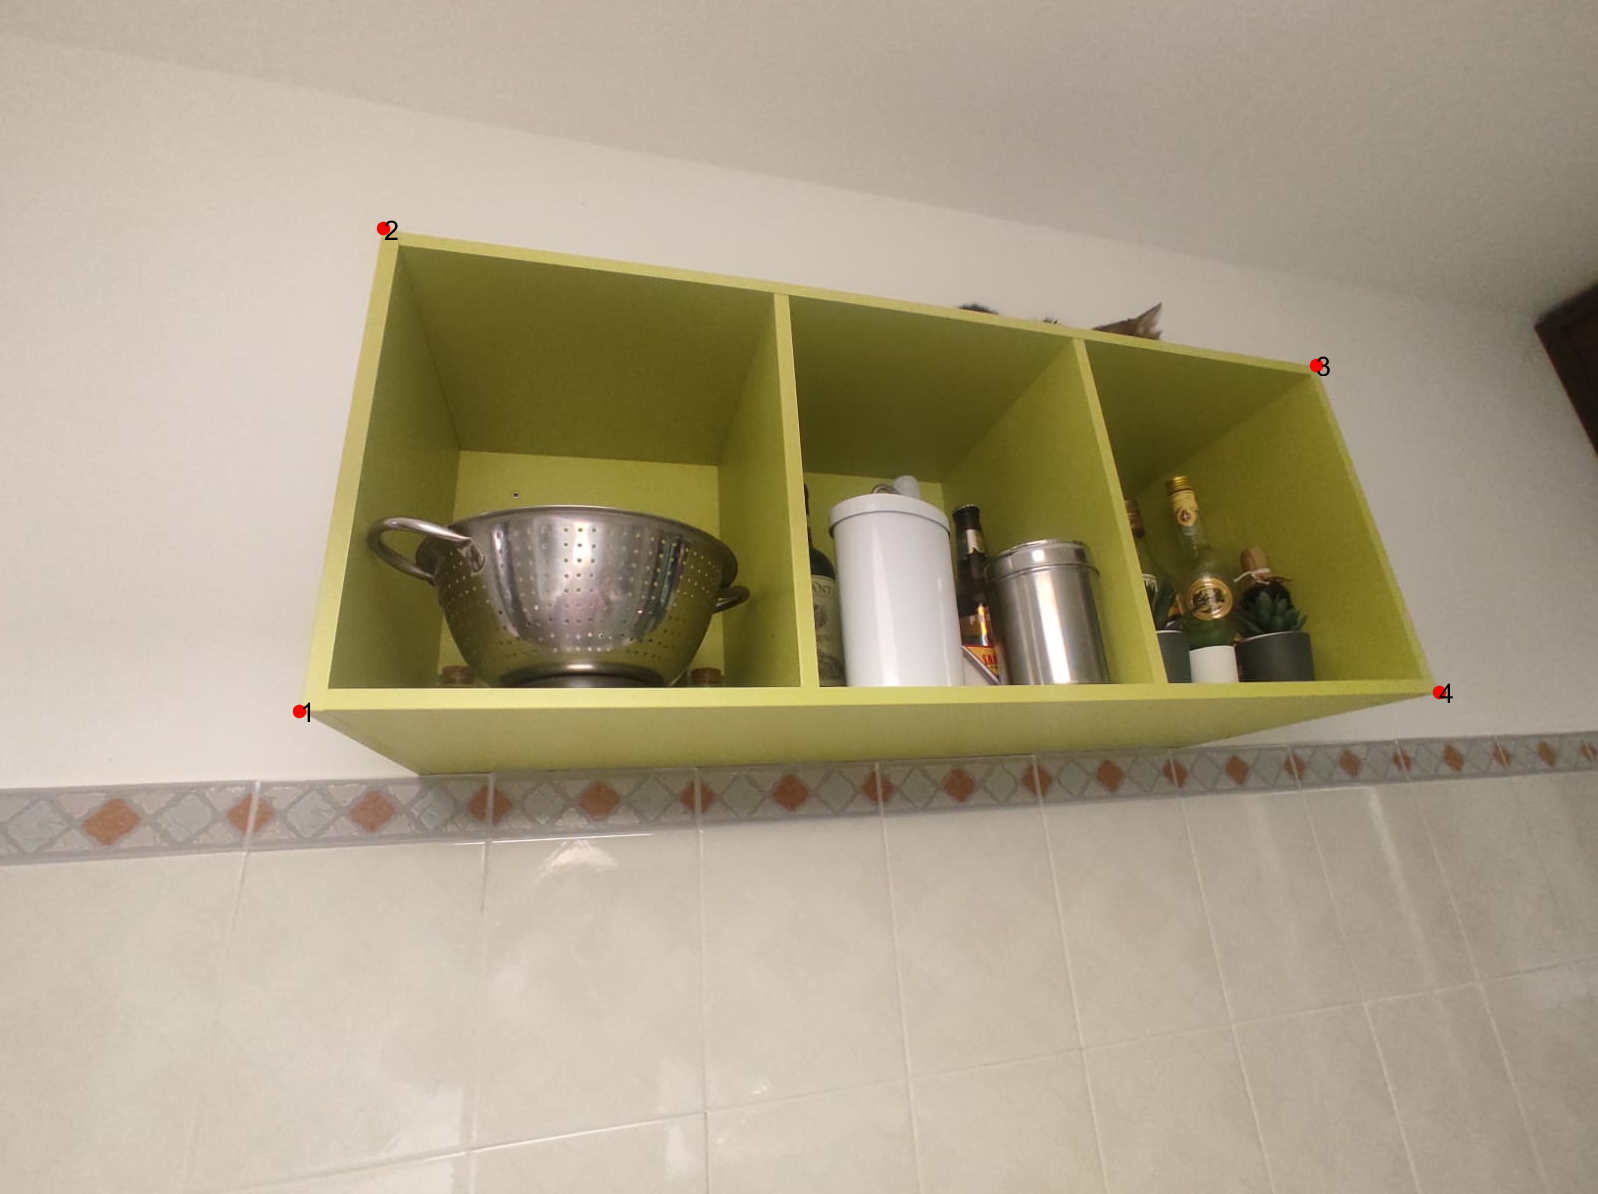
\includegraphics[width=0.5\linewidth]{images/world.png}
    \caption{Vertical facade vertices that forms a plane}
    \label{fig:world}
\end{figure}
The first step was to identify the mapping between the reconstructed image points in metric space and the new world reference frame defined by the plane $\pi$. 
With this, any point in the rectified image could be mapped to the world frame using the equation:
\begin{equation}
\begin{bmatrix}
    \mathbf{R}_\pi \mid \mathbf{o}_\pi 
\end{bmatrix}
\end{equation}
Here, $\mathbf{X}_\pi$ represents a point on the plane in homogeneous coordinates:
\begin{equation}\mathbf{X}_\pi = \begin{bmatrix} 
0 \\ y \\ z \\ w
\end{bmatrix} \end{equation}
The transformation from 3D points in the world space $\mathbf{X}$ to image points $\mathbf{x}$ is given by the projection matrix $\mathbf{P}$:
\begin{equation} 
\mathbf{P} = \begin{bmatrix}
    \mathbf{KR} \mid -\mathbf{KR}_o 
\end{bmatrix}
\end{equation}
where $\mathbf{R}$ is the rotation matrix describing the orientation of the camera with respect to the world frame, and $\mathbf{o}_\pi$ is the camera's position in Cartesian coordinates.
The relationship between image points and 3D world points is:
\begin{equation}\mathbf{x}=\mathbf{PX}\end{equation}
Using this projection mapping, the following relationship was derived:

\begin{equation}
\mathbf{U} =\begin{bmatrix}
    \mathbf{K} \mid  \mathbf{0}
\end{bmatrix}
\begin{bmatrix}
    \mathbf{j}_\pi & \mathbf{k}_\pi & \mathbf{o}_\pi \\ 0 & 0 & 1
\end{bmatrix}
\begin{bmatrix}
    y & z & w
\end{bmatrix}
\end{equation}
Here, the parameters $\mathbf{j}_\pi$, $\mathbf{k}_\pi$, and $\mathbf{o}_\pi$ represent the basis vectors and the origin of the world frame. 
These parameters were derived from the homography $\mathbf{H}$, which maps real-world points to image coordinates:
\begin{equation}\mathbf{K}\begin{bmatrix}
    \mathbf{j}_\pi \mid \mathbf{k}_\pi \mid \mathbf{o}_\pi
\end{bmatrix}=\mathbf{H}\end{equation}
Given the known shape and size of the horizontal face in the world, $\mathbf{H}$ was known, allowing the calculation of:
\begin{equation}\begin{bmatrix}
    \mathbf{j}_\pi \mid \mathbf{k}_\pi \mid \mathbf{o}_\pi
\end{bmatrix} = \mathbf{K}^{-1}\mathbf{H} \end{equation}
Next, the rotation matrix $\mathbf{R}$ that describes the orientation of the plane $\pi$ relative to the camera was computed using the following set of equations:
\begin{equation}\begin{cases}
    \lambda = \frac{1}{\lvert \mathbf{K}^{-1} \mathbf{h}_1 \rvert} \\
    \mathbf{j}_\pi = \mathbf{K}^{-1} \mathbf{h}_1 \lambda \\
    \mathbf{k}_\pi = \mathbf{K}^{-1} \mathbf{h}_2 \lambda \\
    \mathbf{i}_\pi = \mathbf{j}_\pi \times \mathbf{k}_\pi \\
    \mathbf{o}_\pi = \mathbf{K}^{-1} \mathbf{h}_3 \lambda
\end{cases}\end{equation}
Here, $\mathbf{h}_1$, $\mathbf{h}_2$, and $\mathbf{h}_3$ are the columns of the homography $\mathbf{H}$. The scalar $\lambda$ is a normalization factor ensuring the proper scale for the vectors.

Due to noise in the data, the rotation matrix $\mathbf{R}$ may not be perfectly orthogonal. 
To resolve this, SVD was applied to approximate an orthogonal matrix for $\mathbf{R}$, yielding:
\begin{equation}\mathbf{R} = \mathbf{UV} \end{equation}

\paragraph*{MATLAB}
The MATLAB implementation of this procedure can be found in the script located at: \\ 
\texttt{src/image\_analysis/2\_theory\_implementation/6\_localization/main.m} \\
In this script, all the necessary variables mentioned above were imported, and the metric transformation was applied to the image points.

Once the transformation was applied, the world reference frame was defined, and the mapping between the world and image coordinates was computed, considering the translation from the image to the world frame.

With the homography in hand, the previously derived relationships were used to extract the camera's rotation and position matrices. 
The camera's position relative to the reference frame was found to be:
\begin{equation}\text{cameraPosition}=\begin{bmatrix}
    185.8094 \\ -113.9389 \\ 527.3235
\end{bmatrix}\end{equation}
Similarly, the camera's rotation (after SVD orthogonalization) relative to the reference frame was:
\begin{equation} \text{cameraRotation}=\begin{bmatrix} 
    0.9604 & 0.0237 & 0.2774 \\
    -0.0727 & -0.9403 & 0.3324 \\
    0.2688 & -0.3394 & -0.9014
\end{bmatrix}\end{equation}
Figures~\ref{fig:views} show different views of the camera position relative to the object in the world frame. 
In these visualizations, the camera is represented by a red circle, and the three axes indicate the following orientations: \begin{itemize} 
    \item \textit{Red} ($x$): points to the horizontal direction of the camera. 
    \item \textit{Green} ($y$): points downward along the vertical axis of the camera. 
    \item \textit{Blue} ($z$): points in the direction the camera is facing. 
\end{itemize}
\begin{figure}[!htb]
    \centering
    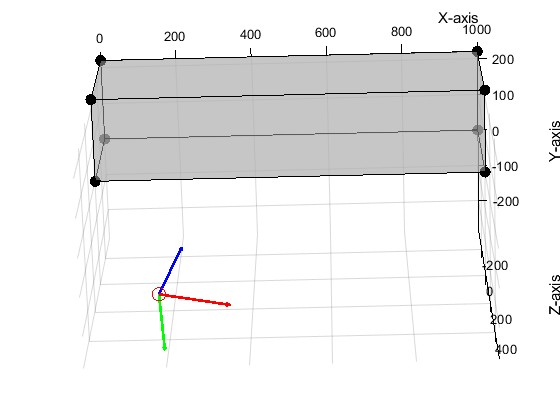
\includegraphics[width=0.5\linewidth]{images/pers.jpg}
    \caption{View of the camera position with respect to the object in world frame}
    \label{fig:views}
\end{figure}
\noindent It’s important to note that the reference frame used here differs slightly from the one initially suggested, as the $y$ and $z$ axes have been swapped. 
This change is purely for visualization purposes, chosen for convenience in representing the main facade as a plane. 
Despite this adjustment, the results remain consistent. 
The swap of these two axes does not affect the final outcome, as the fundamental relationships between the camera and the object are preserved.

\section{Visualization}
The final task involves visualizing the rectified curve and presenting various views of the reconstructed three-dimensional model of the object.

\subsection{Rectified curve visualization}
To visualize the rectified curve, the previously computed homography matrices were utilized to transform specific points along the curve. 
These transformed points were then used to reconstruct the curve's matrix. 
Once the matrix of the rectified curve was determined, the curve was plotted directly onto the rectified image.
Then, we also computed the curve in the vertical reconstructed image in the same way, using the correct homography matrix. 

\paragraph*{MATLAB}
The MATLAB implementation for rectified curve visualization is available in the script located at: \\ 
\texttt{src/image\_analysis/3\_visualization/1\_rectified\_curve\_visualization/main.m} \\
This script leverages the data already computed during earlier steps, including the metric rectification for all points of the image. The following steps summarize the process:
\begin{enumerate}
    \item Import the necessary data, including homography matrices and the curve $\mathbf{S}$ points.
    \item Apply the computed transformations to the image and the curve points to rectify them.
    \item Use the \texttt{conic\_extractor} function to derive the rectified curve’s matrix from the transformed points.
    \item Plot the resulting rectified curve onto the metric rectified image.
\end{enumerate}
The result, as shown in Figure~\ref{fig:curve_ext}, demonstrates the rectified curve.
The rectified curve $\mathbf{S}$ closely resembles a perfect circumference, which aligns with the expectations and validates the accuracy of the applied transformations.

For the vertical facade reconstruction we have the result shown in Figure \ref{fig:curve_vert}.
\begin{figure}[!htb]
    \centering
    \begin{minipage}{0.49\linewidth}
        \centering
        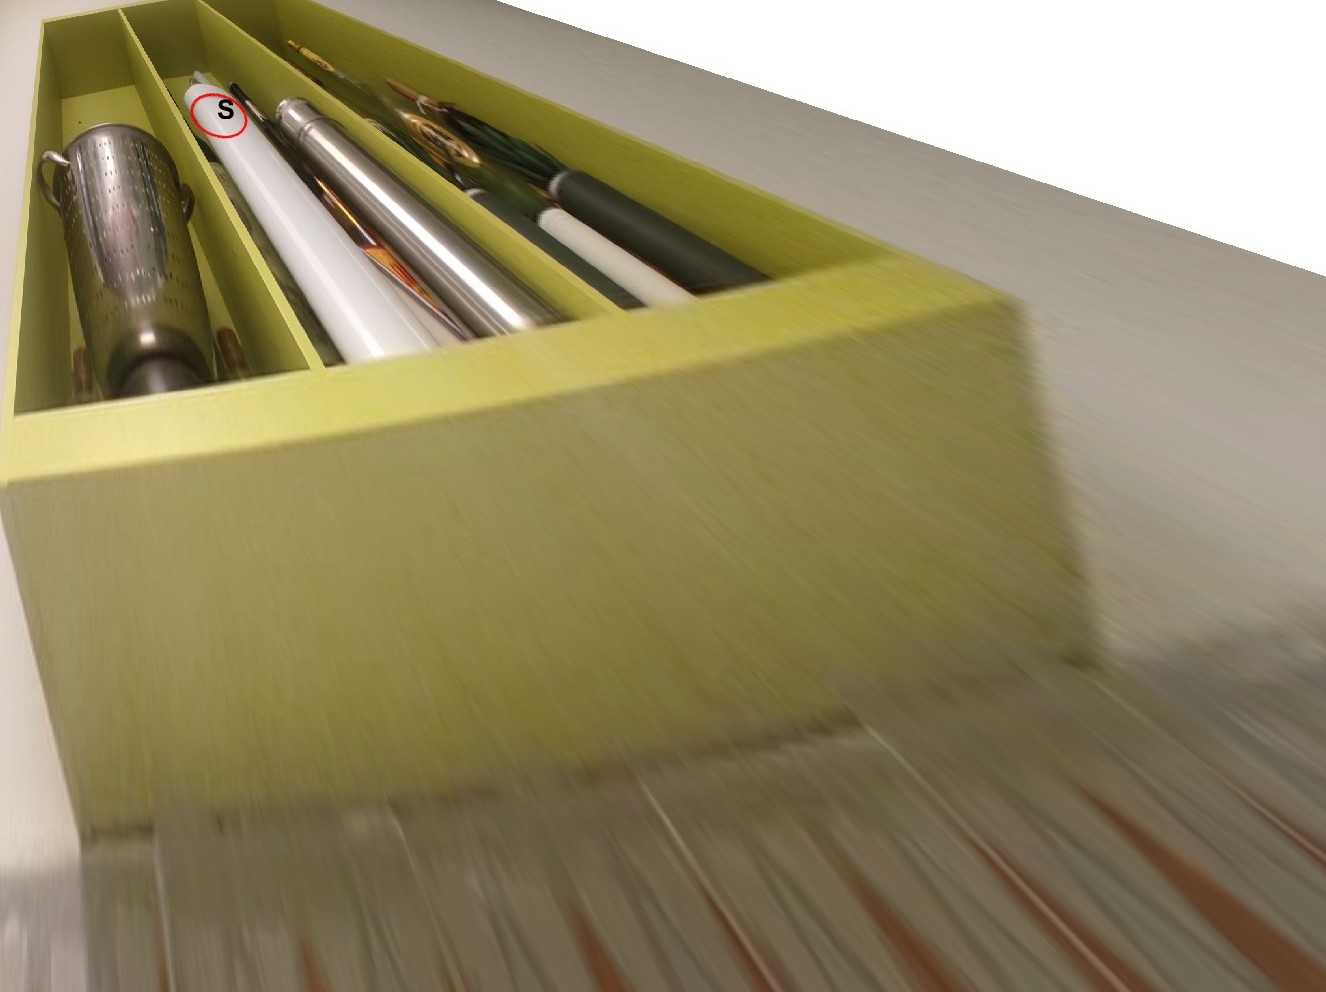
\includegraphics[width=\linewidth]{images/curve_ext.jpg}
        \caption{Rectified curve plotted in the metric rectified image}
        \label{fig:curve_ext}
    \end{minipage}
    \begin{minipage}{0.49\linewidth}
        \centering
        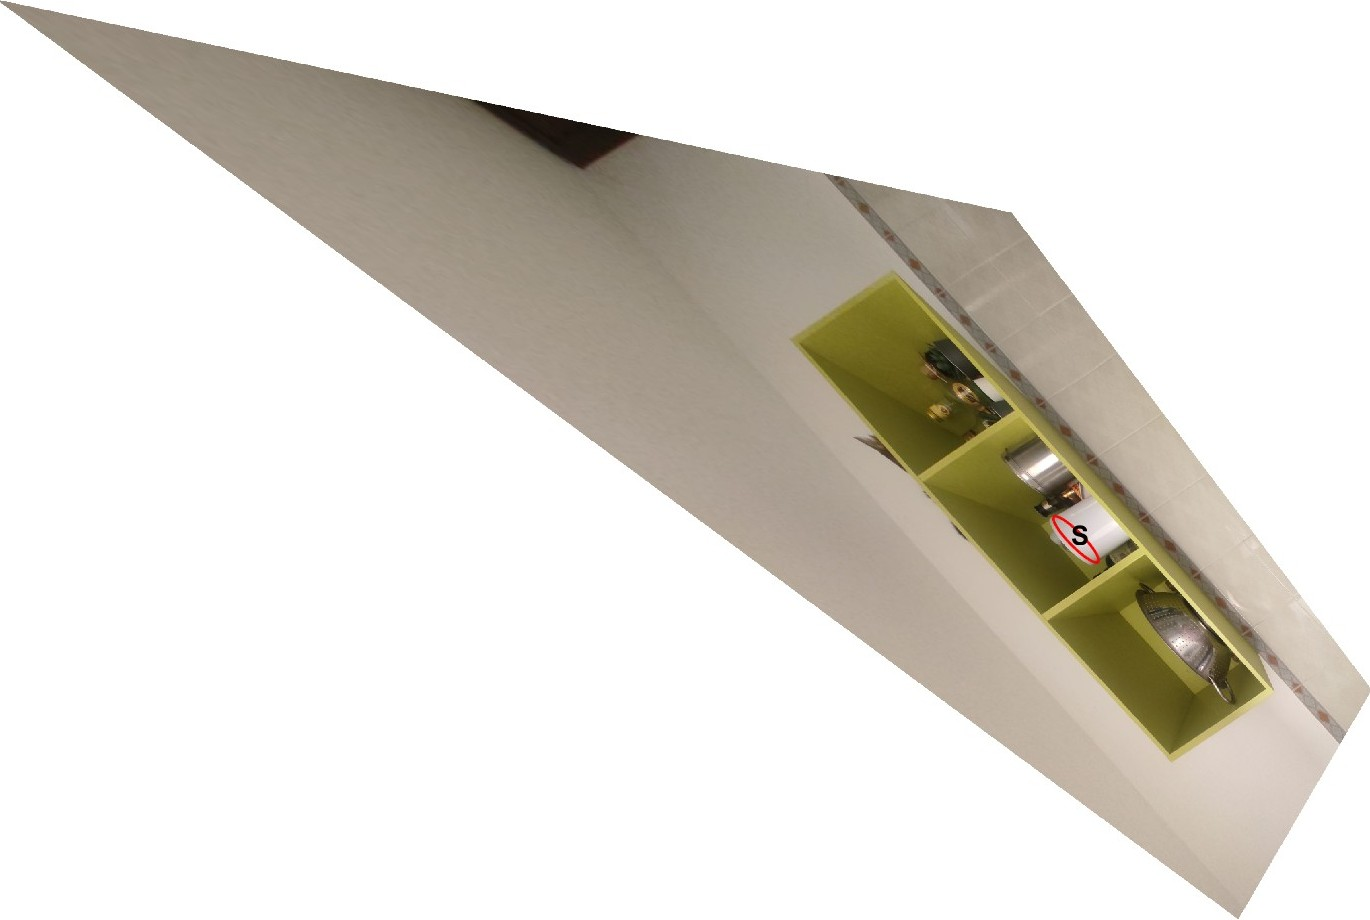
\includegraphics[width=\linewidth]{images/curve_vert.jpg}
        \caption{Rectified curve plotted in the vertical reconstructed image}
        \label{fig:curve_vert}
    \end{minipage}
\end{figure}

\subsection{Three-dimensional visualization}
The second part of the task involved visualizing the reconstructed three-dimensional model of the object along with the camera’s position and orientation.

\paragraph*{MATLAB}
The MATLAB implementation for this task is available in the script located at: \\ 
\texttt{src/image\_analysis/3\_visualization/2\_three\_dimensional\_visualization/main.m} \\
This script utilizes the parameters and transformations computed in previous steps to create a comprehensive three-dimensional representation. 
The process includes:
\begin{enumerate}
    \item Plotting the three-dimensional reference frame, incorporating the object and the camera position.
    \item Ensuring that the camera’s orientation and axes align with the computed parameters.
    \item Capturing visualizations from multiple perspectives to illustrate the spatial relationships between the object and the camera.
\end{enumerate}
The resulting views, shown in Figure~\ref{fig:3dviews}, provide insights into the reconstructed model from different angles.
\begin{figure}[!htb]
    \centering
    \begin{minipage}{0.4\linewidth}
        \centering
        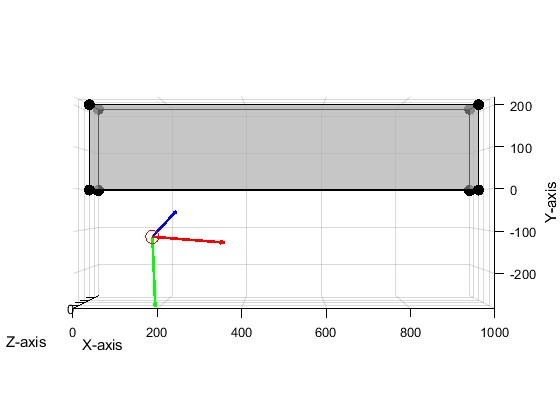
\includegraphics[width=\linewidth]{images/xy.jpg}
        \caption{Front view}
    \end{minipage}%
    \begin{minipage}{0.4\linewidth}
        \centering
        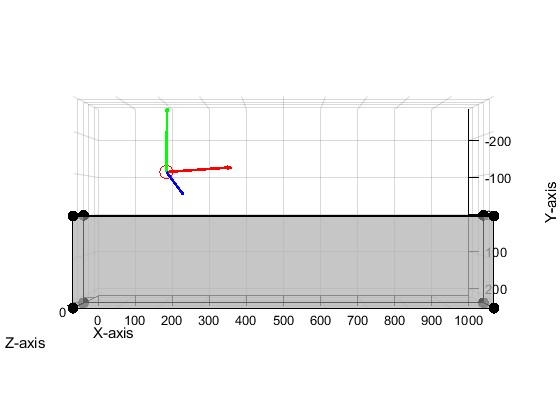
\includegraphics[width=\linewidth]{images/yx.jpg}
        \caption{Rear view}
    \end{minipage}
    
    \begin{minipage}{0.4\linewidth}
        \centering
        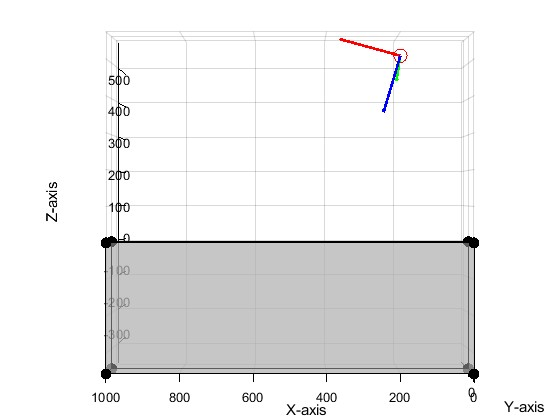
\includegraphics[width=\linewidth]{images/zx.jpg}
        \caption{Top view}
    \end{minipage}%
    \begin{minipage}{0.4\linewidth}
        \centering
        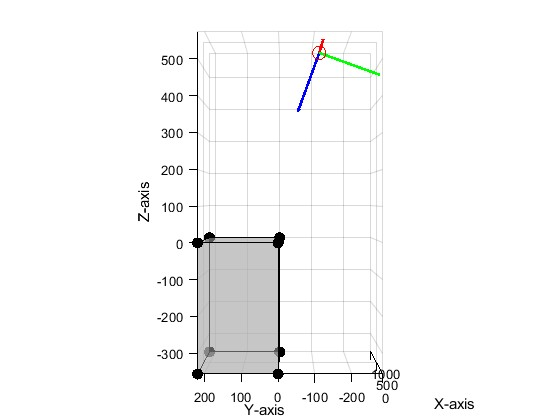
\includegraphics[width=\linewidth]{images/zy.jpg}
        \caption{Lateral view}
    \end{minipage}
    \caption{Multiple views of the camera position and orientation with respect to the reconstructed object in the world frame}
    \label{fig:3dviews}
\end{figure}

The camera’s position and orientation relative to the object are consistent with the initial image, validating the accuracy of the reconstruction process. 
These views highlight how the computed parameters successfully describe the spatial relationship between the object and the camera in the world reference frame.


\section{Additional Information}
All results presented in this report are approximations, aimed at improving readability and simplifying the understanding of the process. 
For more accurate results, the full values and computations are available through the provided scripts and saved variables.
These can be accessed by running the relevant scripts or by checking the stored variables directly. 

\noindent The folder structure and associated scripts are organized as follows:
\renewcommand*\DTstylecomment{\rmfamily\color{blue}\textsc}
\dirtree{%
.1 src.
    .2 image\_analysis\DTcomment{Scripts designed to solve the problems described}.
        .3 1\_feature\_extraction.
            .4 1\_lines\_extraction. 
            .4 2\_curves\_extraction. 
        .3 2\_theory\_implementation.
            .4 1\_vanishing\_line. 
            .4 2\_rectification. 
            .4 3\_calibration. 
            .4 4\_vertical\_reconstruction. 
            .4 5\_curve\_points\_estimation. 
            .4 6\_localization. 
        .3 3\_visualization.
            .4 1\_rectified\_curve\_visualization. 
            .4 2\_three\_dimensional\_visualization. 
    .2 images\DTcomment{Directory containing the resulting images}.
    .2 utils\DTcomment{Utility functions shared by various scripts}.
    .2 variables\DTcomment{Folder containing variables with the computed results}.
}
Each sub-folder within \texttt{1\_feature\_extraction}, \texttt{2\_theory\_implementation}, and \\ \texttt{3\_visualization} contains a single script, \texttt{main.m}.
Running this script will compute all necessary variables and transformations required for each corresponding step of the process.

The primary folder to focus on for executing all the scripts is \texttt{src}. 
It contains essential sub-folders, such as those for images, variables, and utility functions, which are needed to perform the computations and generate the results.

All the information used to complete this homework was sourced from the recommended book \cite{book} and the lecture slides \cite{slides}.

\singlespacing
\emergencystretch 3em
\hfuzz 1px
\printbibliography[heading=bibnumbered]

\end{document}